\section*{五、双曲线}
\section{双曲线及其标准方程}
我们知道，平面内与两定点$F_1,F_2$的距离之和为常数（常数$>|F_1F_2|$）的点的轨迹是椭圆，那么与这两定点的距离的差为常数的点的轨迹又是怎样的曲线？

在画图板上（板上放一张白纸）钉两个钉子作为两个定点$F_1$、$F_2$．取长度之差为$2a$的两条线，把长的一端系在$F_1$上，把短的一端系在$F_2$上，它们的另一端打成结$M$. 以铅笔尖套住这两条线，左手将结$M$轻轻拉紧，右手握笔顺势移动，则笔尖$P$在纸上画出的图形就是曲线的一支. 而且这样画出的曲线，不论点$P$移动到什么位置，$PF_1$与$PF_2$长度之差总为$2a$，事实上
\[|PF_1|-|PF_2|=(|PF_1|+|PM|)-(|PF_2|+|PM|)=\text{两线长度的差}=2a\]

如果把两条线绳交换位置，同样的方法可以画出曲线的另一支（图3.26）．

\begin{thm}
 {定义} 平面内与两个定点$F_1$、$F_2$的距离的差的绝对值是常数（小于$|F_1F_2|$）的点的轨迹叫做\textbf{双曲线}. 这两个定点叫做双曲线的\textbf{焦点}、两焦点的距离叫做\textbf{焦距}.   
\end{thm}

取过焦点$F_1$、$F_2$的直线为$x$轴，线段$F_1F_2$的垂直平分线为$y$轴（如图3.27）．


\noindent
\begin{minipage}{.45\textwidth}
    \centering
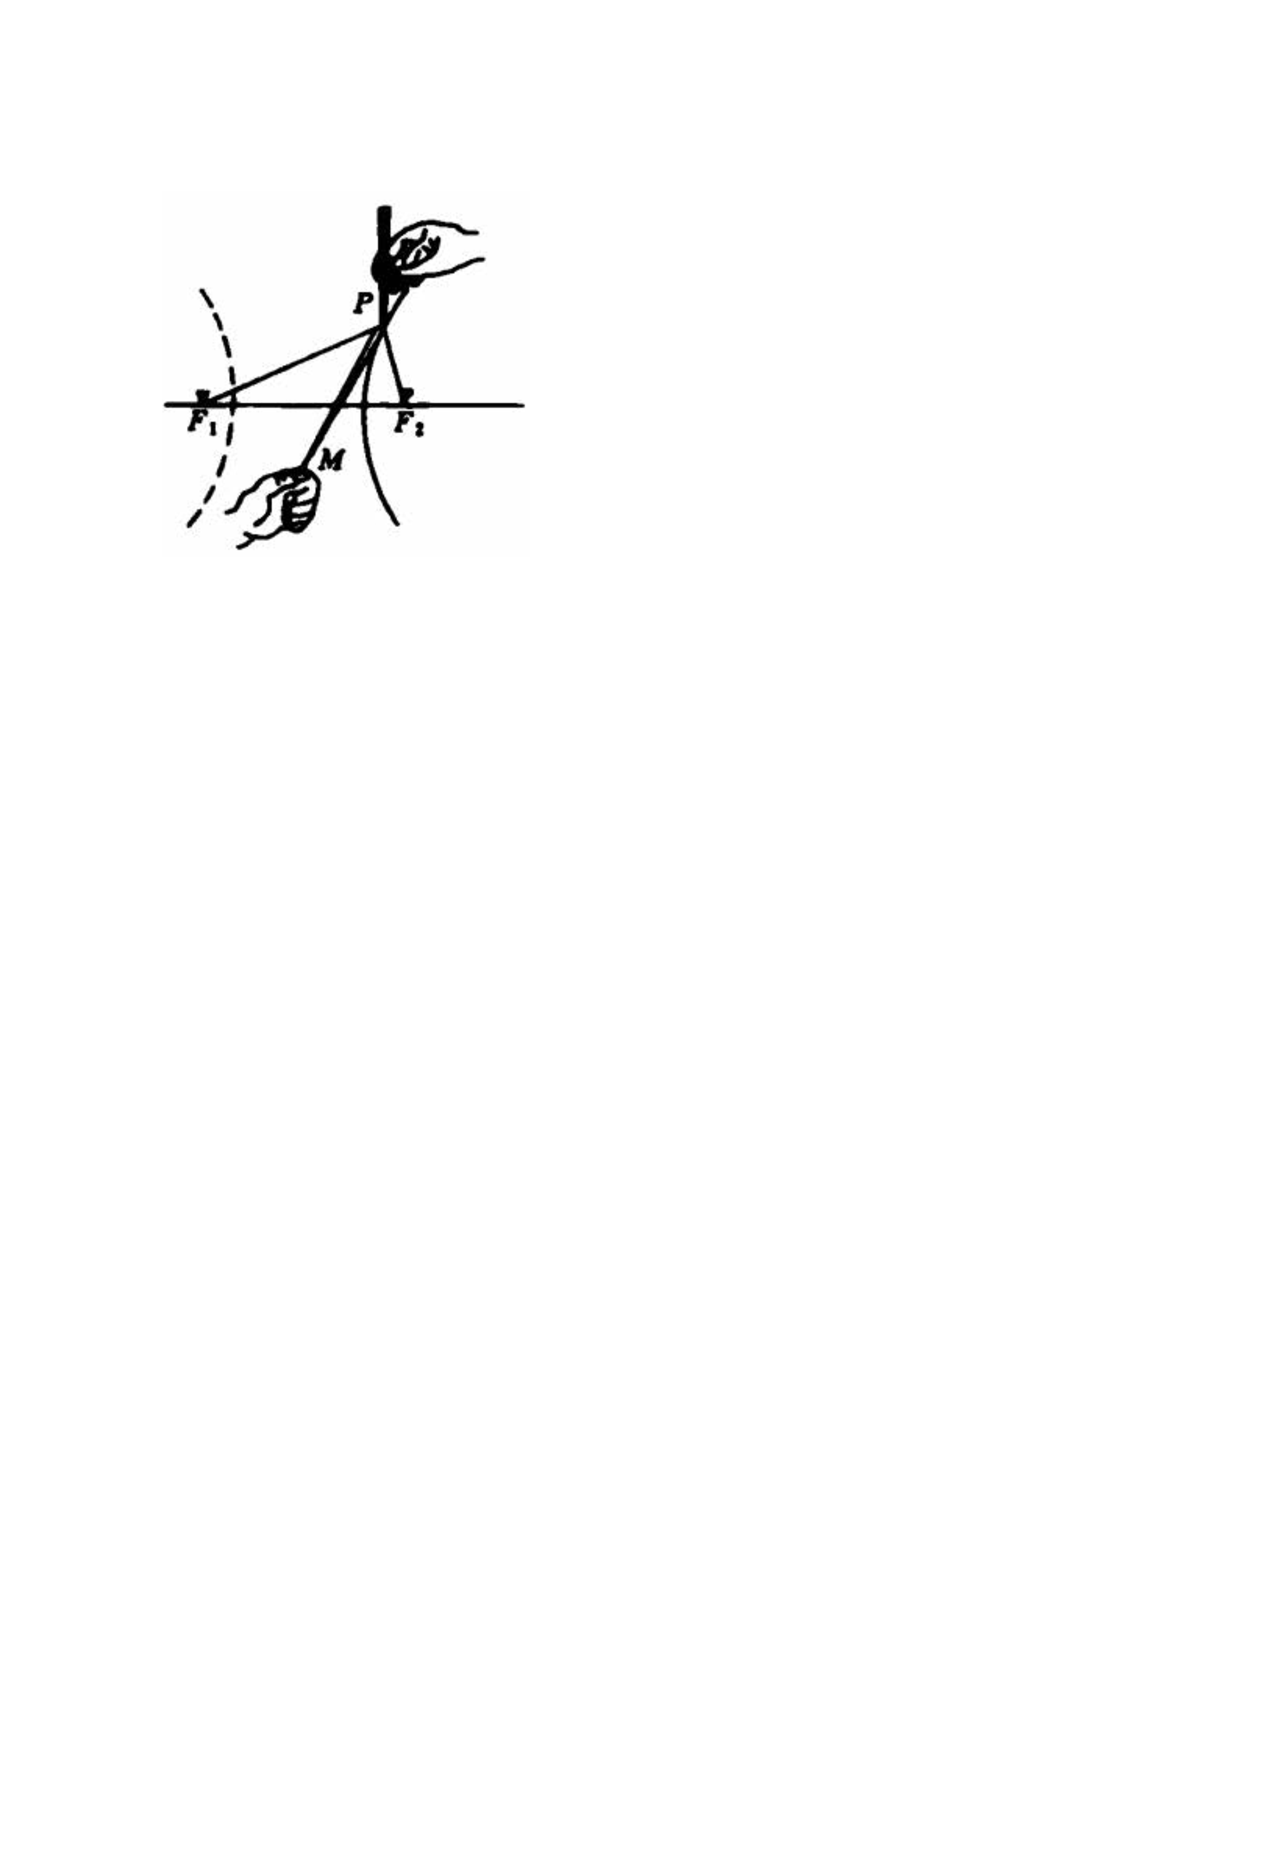
\includegraphics[scale=.9]{fig/3-26.pdf}
\captionof{figure}{}
\end{minipage}
\hfill
\begin{minipage}{.45\textwidth}
\centering
\begin{tikzpicture}[>=stealth, scale=.9]
\draw[->](-3,0)--(3,0)node[below]{$x$};
\draw[->](0,-3)--(0,3)node[left]{$y$};
\node[below left]{$O$};
\draw[domain=-2:2, smooth, thick]plot({sqrt(\x*\x+1)},\x);
\draw[domain=-2:2, smooth, thick]plot({-sqrt(\x*\x+1)},\x);
\tkzDefPoints{-1.414/0/F_1, 1.414/0/F_2, 1.5/1.12/P}
\draw[dashed](F_1)--(P)--(F_2);
\tkzLabelPoints[below](F_1,F_2)
\tkzLabelPoints[right](P)
\tkzDrawPoints(P,F_1,F_2)
\end{tikzpicture}
\captionof{figure}{}
\end{minipage}


设$P(x,y)$是双曲线上的任意一点，双曲线的焦距是$2c\; (c>0)$，那么$F_1$、$F_2$的坐标分别是$(-c,0)$、$(c,0)$. 又设点$P$与$F_1$和$F_2$的距离的差的绝对值等于常数$2a$．

$\because\quad \Big||PF_1|-|PF_2|\Big|=2a$

$\therefore\quad |PF_1|-|PF_2|=\pm 2a\quad \Rightarrow\quad \sqrt{(x+c)^2+y^2}-\sqrt{(x-c)^2+y^2}=\pm 2a$

化简，得
\[(c^2-a^2)x^2-a^2y^2=a^2(c^2-a^2)\]

由双曲线的定义，$2c>2a$，即$c>a$，所以$c^2-a^2>0$，设$c^2-a^2=b^2\; (b>0)$，代入上式得
\[b^2x^2-a^2y^2=a^2b^2\]
也就是
\begin{equation}
    \frac{x^2}{a^2}-\frac{y^2}{b^2}=1 \tag{1}
\end{equation}

可以证明，坐标满足方程的点也在曲线上.


\noindent
\begin{minipage}{.52\textwidth}
\CTEXindent

这个方程叫做\textbf{双曲线的标准方程}，它所表示的双曲线的焦点在$x$轴上，焦点是$F_1(-c,0),\; F_2(c,0)$，这里$c^2=a^2+b^2$.

如果双曲线的焦点在$y$轴上（图3.28），焦点是$F_1(0,-c)$、$F_2(0,c)$，只要将方程（1）的$x$、$y$互换就可以得到它的方程
\[\frac{y^2}{a^2}-\frac{x^2}{b^2}=1\]

这个方程也是双曲线的标准方程.
\end{minipage}
\hfill
\begin{minipage}{.45\textwidth}
\centering
\begin{tikzpicture}[>=stealth, scale=1]
\draw[->](-2.5,0)--(2.5,0)node[below]{$x$};
\draw[->](0,-2.5)--(0,2.5)node[left]{$y$};
\node[below left]{$O$};
\draw[domain=-2:2, smooth, thick]plot(\x, {sqrt(\x*\x+1)});
\draw[domain=-2:2, smooth, thick]plot(\x, -{sqrt(\x*\x+1)});
\tkzDefPoints{0/-1.414/F_1, 0/1.414/F_2, -1.12/-1.5/M}
\draw[dashed](F_1)--(M)--(F_2);
\tkzLabelPoints[right](F_1,F_2)
\tkzLabelPoints[left](M)
\tkzDrawPoints(M,F_1,F_2)
\end{tikzpicture}
\captionof{figure}{}
\end{minipage}

\begin{figure}[htp]
    \centering
    \caption*{椭圆与双曲线的标准方程的对比}
\begin{tabular}{c|c|c}
    \hline
    & 椭圆 & 双曲线\\
\hline
几何条件 &  $|PF_1|+|PF_2|=2a$    &   $\Big||PF_1|-|PF_2|\Big|=2a$    \\ \hline
$a,b,c$ &   $a^2=b^2+c^2$   &  $c^2=a^2+b^2$     \\
之间的关系 &  ($a>c>0,\; a>b>0$)    &    ($c>a>0,\; c>b>0$)   \\[1.5ex]  \hline
标准方程 &  $\frac{x^2}{a^2}+\frac{y^2}{b^2}=1,\quad \frac{x^2}{b^2}+\frac{y^2}{a^2}=1$    &   $\frac{x^2}{a^2}-\frac{y^2}{b^2}=1,\quad \frac{y^2}{a^2}-\frac{x^2}{b^2}=1$    \\[1.5ex] \hline
焦点位置 &  看方程中含$x^2,y^2$项的    &   看方程中含$x^2,y^2$项的正负    \\
& 分母的大小& （与分母的大小无关）\\
\hline
\end{tabular}
\end{figure}

\begin{example}
    已知两点$F_1(0,-5)$、$F_2(0,5)$，求与它们的距离的差的绝对值是6的点的轨迹方程．
\end{example}

\begin{solution}
按双曲线的定义，所求点的轨迹是双曲线，且$F_1$、$F_2$
是此双曲线的焦点.

$\because\quad c=5,\quad a=3$

$\therefore\quad b^2=c^2-a^2=16$.

又$\because\quad $双曲线的两焦点在$y$轴上，

$\therefore\quad $所求轨迹方程为$\frac{y^2}{9}-\frac{x^2}{16}=1$.
\end{solution}


\begin{example}
    $k$为何值时，方程$\frac{x^2}{9-k}+\frac{y^2}{k-1}=1$的曲线是双曲线？并写出相应的焦点坐标.
\end{example}

\begin{solution}
    当$k<1$时，方程变为$\frac{x^2}{9-k}-\frac{y^2}{1-k}=1$.

$\because\quad a^2=9-k,\quad b^2=1-k$

$\therefore\quad c^2=a^2+b^2=10-2k$

方程表示以$F_1(-\sqrt{10-2k},0)$、$F_2(\sqrt{10-2k},0)$为焦点、$2a=2\sqrt{9-k}$的双曲线.

当$k>9$时，方程变为$\frac{y^2}{k-1}-\frac{x^2}{k-9}=1$

$\because\quad a^2=k-1,\quad b^2=k-9$

$\therefore\quad c^2=a^2+b^2=2k-10$

方程表示以$F_1(0,-\sqrt{2k-10})$、$F_2(0,\sqrt{2k-10})$为焦点、$2a=2\sqrt{k-1}$的双曲线.
\end{solution}

\subsection*{3.11 练习}
\begin{enumerate}
\item 求适合下列条件的双曲线的标准方程：
\begin{enumerate}[(1)]
\item $a=4$, $b=3$，焦点在$x$轴上；
\item $a=2\sqrt{5}$，经过点$A(2,-5)$，焦点在$y$轴上．
\end{enumerate}

\item 证明：椭圆$\frac{x^2}{25}+\frac{y^2}{9}=1$与双曲线$x^2-15y^2=15$的焦点相
同.
\item 平面内，与两定点$F_1, F_2$距离之差的绝对值等于$|F_1F_2|$的动点$P$的轨迹是什么图形？   
\end{enumerate}

\section{双曲线的几何性质}
我们可根据双曲线的标准方程$\frac{x^2}{a^2}-\frac{y^2}{b^2}=1$
得出双曲线的几何性质.
\begin{enumerate}
    \item 几何特性：
    若点$P$在双曲线$\frac{x^2}{a^2}-\frac{y^2}{b^2}=1$上，则
    \[\Big||PF_1|-|PF_2|\Big|=2a\]
    其中$F_1(-c,0)$、$F_2(c,0)$是双曲线的焦点．
    \item 范围：
    由于$x\in(-\infty,-a]\cup [a,+\infty)$, $y\in\R$. 说明双曲线在两条直线$x=a$、$x=-a$的外侧.
    \item 对称性：
    双曲线$\frac{x^2}{a^2}-\frac{y^2}{b^2}=1$关于$x$轴、$y$轴及原点$O$对称（原点$O$叫做双曲线的中心）.
    \item 顶点：双曲线$\frac{x^2}{a^2}-\frac{y^2}{b^2}=1$与其对称轴的交点$A_1(-a,0)$、$A_2(a,0)$叫做双曲线的顶点.
    \item 离心率：$e=\frac{c}{a}>1$
    \item 实轴和虚轴：

\noindent
\begin{minipage}{.5\textwidth}
    令$x=0$，得$y^2=-b^2$. 这个方程没有实数根，说明双曲线$\frac{x^2}{a^2}-\frac{y^2}{b^2}=1$和$y$轴没有交点，但我们也把$B_1(0,-b)$, $B_2(0,b)$画在$y$轴上（如图3.29）．

    线段$A_1A_2$叫做双曲线的\textbf{实轴}，它的长等于$2a$，$a$叫做双曲线的\textbf{实半轴长}. 线段$B_1B_2$叫做双曲线的\textbf{虚轴}，它的长等于$2b$，$b$叫做双曲线的\textbf{虚半轴长}．实轴和虚轴等长的双曲线叫做\textbf{等轴双曲线}.
\end{minipage}
\hfill
\begin{minipage}{.45\textwidth}
\centering
\begin{tikzpicture}[>=stealth, scale=.9]
\draw[->](-2.5,0)--(2.5,0)node[below]{$x$};
\draw[->](0,-2.5)--(0,2.5)node[left]{$y$};
\node[below left]{$O$};
\draw[domain=-2:2, smooth, thick]plot({sqrt(\x*\x+1)},\x);
\draw[domain=-2:2, smooth, thick]plot({-sqrt(\x*\x+1)},\x);
\tkzDefPoints{-1.414/0/F_1, 1.414/0/F_2}
\draw[dashed](-1,-1)rectangle (1,1);
\tkzLabelPoints[below](F_1,F_2)
\tkzDrawPoints(F_1,F_2)
\draw[thick](0,1)node[above right]{$B_2$}--(1,0)node[below left]{$A_2$};
\node at (0,-1)[below right]{$B_1$};
\node at (-1,0)[above right]{$A_1$};
\end{tikzpicture}
\captionof{figure}{}
\end{minipage}

\item 双曲线的渐近线：

    由于双曲线不是封闭曲线，因此，如何描述曲线向无穷远延伸时的趋势，是我们应解决的问题.

$\because\quad \frac{x^2}{a^2}-\frac{y^2}{b^2}=1$

$\therefore\quad y=\pm\frac{b}{a}\sqrt{x^2-a^2}=\pm\frac{b}{a}|x|\cdot \sqrt{1-\frac{a^2}{x^2}}=\pm\frac{bx}{a}\sqrt{1-\left(\frac{a}{x}\right)^2}$

当$x\to \infty$时，有$y\to \pm\frac{b}{a}x$.

这就使我们可以这样认为，当双曲线向无穷远延伸时，逐
渐逼近直线$y=\pm\frac{b}{a} x$.
\end{enumerate}

经过$A_2$、$A_1$作$y$轴的平行线$x=\pm a$，经过$B_2$、$B_1$作$x$轴的平行线$y=\pm b$，四条直线围成一个矩形（图3.30）．矩形的两条对角线所在直线的方程是$y=\pm\frac{b}{a}x$，双曲线$\frac{x^2}{a^2}-\frac{y^2}{b^2}=1$的各支向外延伸时，与这两条直线逐渐接近.

下面引入曲线的渐近线的概念：

若曲线能延伸到无穷远，而动点$P$沿着曲线向无穷远移动时，它与某一定直线的距离趋于零，则称这条直线是曲线的一条\textbf{渐近线}.

为了证明直线$y=\pm\frac{b}{a}x$是双曲线$\frac{x^2}{a^2}-\frac{y^2}{b^2}=1$的渐近线，由双曲线的对称性，我们只需证明曲线在第一象限时的情形.

\noindent
\begin{minipage}{.5\textwidth}
\centering
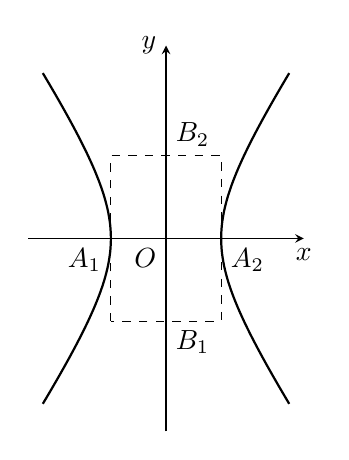
\begin{tikzpicture}[>=stealth, scale=.7]
\draw[->](-2.5,0)--(2.5,0)node[below]{$x$};
\draw[->](0,-3.5)--(0,3.5)node[left]{$y$};
\node[below left]{$O$};
\draw[domain=-3:3, smooth, thick]plot({sqrt(0.444*\x*\x+1)},\x);
\draw[domain=-3:3, smooth, thick]plot({-sqrt(0.444*\x*\x+1)},\x);
\draw[dashed](-1,-1.5)rectangle (1,1.5);
\node at (0,1.5)[above right]{$B_2$};
\node at (1,0)[below right]{$A_2$};
\node at (0,-1.5)[below right]{$B_1$};
\node at (-1,0)[below left]{$A_1$};
\tkzDefPoints{-1/1.5/H,1/1.5/G,-1/-1.5/E,1/-1.5/F}
\tkzDrawLines[add =.6 and .6](F,H E,G)
\tkzLabelPoints[below](E,F)
\tkzLabelPoints[above](G,H)
\end{tikzpicture}
\captionof{figure}{}
\end{minipage}
\hfill
\begin{minipage}{.45\textwidth}
\centering
\begin{tikzpicture}[>=stealth]
\draw[->](-1,0)--(4,0)node[below]{$x$};
\draw[->](0,-1)--(0,3)node[left]{$y$};
\node[below right]{$O$};
\draw[domain=0:2.5, smooth, thick]plot({sqrt(1.5625*\x*\x+1)},\x)node[below right]{$P(x,y)$};
\draw[dashed](0,.8)node[left]{$B_2$}--(1,.8)node[above]{$G$}--(1,0)node[below]{$A_2$};
\tkzDefPoints{0/0/O, 1/.8/G}
\tkzDrawLines[add =1 and 2.5](O,G)

\end{tikzpicture}
\captionof{figure}{}
\end{minipage}


设位于第一象限的双曲线上的动点$P$的坐标为$(x,y)$（图3.31），则
\[y=\frac{b}{a}\sqrt{x^2-a^2}\]

$P$点到直线$bx-ay=0$的距离$d$为
\[\begin{split}
    d=\frac{|bx-b\sqrt{x^2-a^2}|}{\sqrt{b^2+a^2}}&=\frac{b\left(x-\sqrt{x^2-a^2}\right)}{\sqrt{b^2+a^2}}\\
    &=\frac{b[x^2-(x^2-a^2)]}{\sqrt{b^2+a^2}\left(x+\sqrt{x^2-a^2}\right)}\\
    &=\frac{ba^2}{\sqrt{b^2+a^2}}\cdot \frac{1}{x+\sqrt{x^2-a^2}}
\end{split}\]

$\because\quad $当$x\to +\infty$时，$\frac{1}{x+\sqrt{x^2-a^2}}\to 0$

$\therefore\quad d\to 0$

$\therefore\quad $直线$y=\frac{b}{a}x$是双曲线的一条渐近线. 同理可证$y=-\frac{b}{a}x$也是双曲线的一条渐近线.

对于给定的双曲线$\frac{x^2}{a^2}-\frac{y^2}{b^2}=1$，如何求它的渐近线方程？

$\because\quad y=\pm\frac{b}{a}x$可写成$\frac{x}{a}\pm\frac{y}{b}=0$

而\[\left(\frac{x}{a}+\frac{y}{b}\right)\left(\frac{x}{a}-\frac{y}{b}\right)=0\]
即
\[\frac{x^2}{a^2}-\frac{y^2}{b^2}=0\]

因此，只要将双曲线方程$\frac{x^2}{a^2}-\frac{y^2}{b^2}=1$中等号右边的常数1改为0后，即为此双曲线渐近线的方程．

有了双曲线的渐近线，双曲线的作图就能比较准确，今后画双曲线，一般都应画出它的渐近线.

\begin{example}
    求双曲线$9y^2-16x^2=144$的实半轴长和虚半轴长、焦点坐标、离心率、渐近线方程.
\end{example}

\begin{solution}
把方程化为标准方程
\[\frac{y^2}{4^2}-\frac{x^2}{3^2}=1\]
由此可知，实半轴长$a=4$，虚半轴长$b=3$.
\[c=\sqrt{a^2+b^2}=\sqrt{4^2+3^2}=5\]

焦点的坐标是$(0,-5)$，$(0,5)$．

离心率$e=\frac{c}{a}=\frac{5}{4}$.

渐近线方程为$x=\pm\frac{3}{4}y$，即$y=\pm \frac{4}{3}x$.
\end{solution}


\begin{example}
双曲线型自然通风塔的外形，是双曲线的一部分绕其虚轴旋转所成的曲面（图3.32），它的最小半径为12米，上口半径为13米，下口半径为25米，高55米．在所给的坐标系中求此双曲线的方程.
\end{example}

\begin{figure}[htp]
\begin{minipage}{.45\textwidth}
 \centering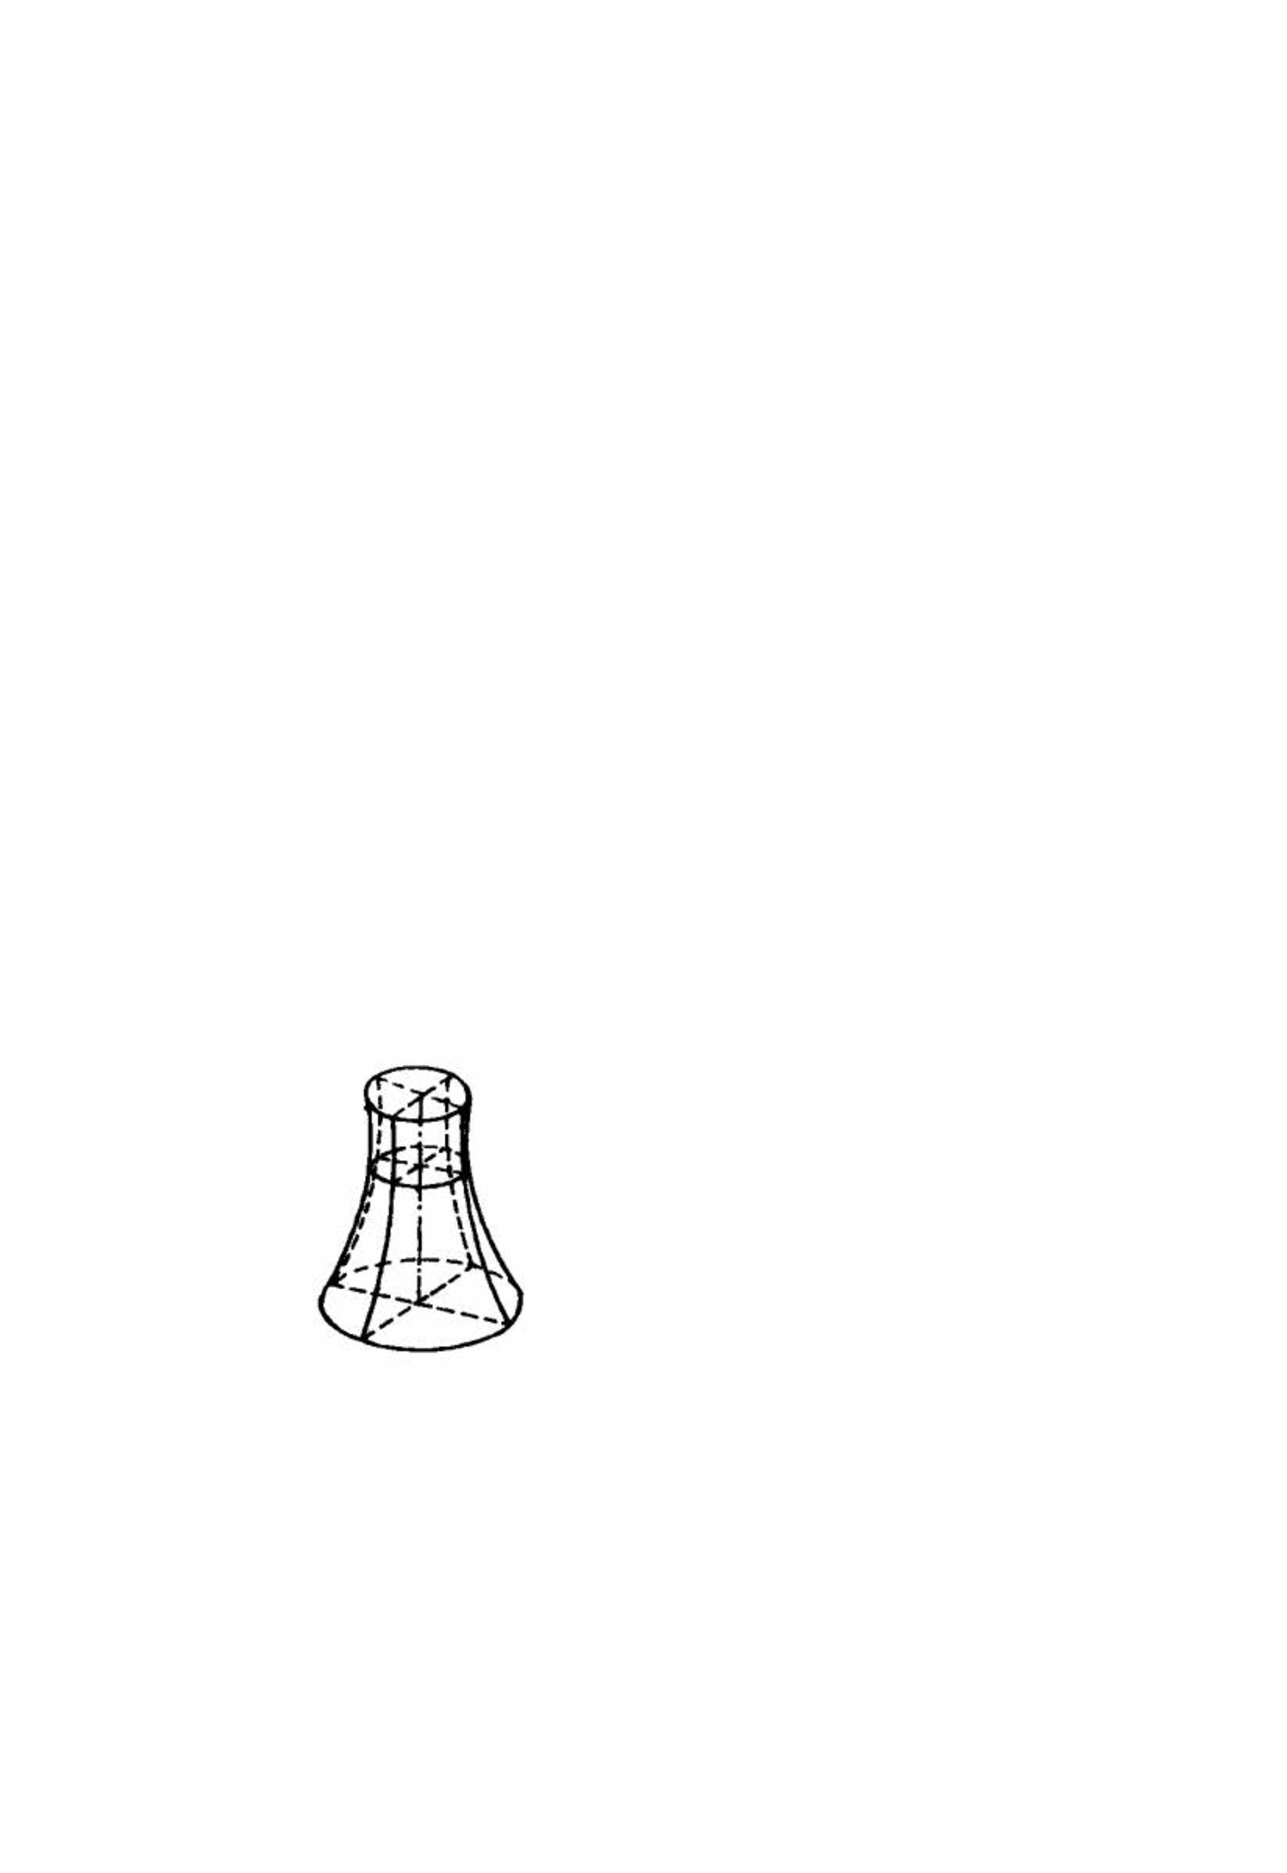
\includegraphics{fig/3-32.pdf}
\end{minipage}
\hfill
\begin{minipage}{.45\textwidth}
\centering
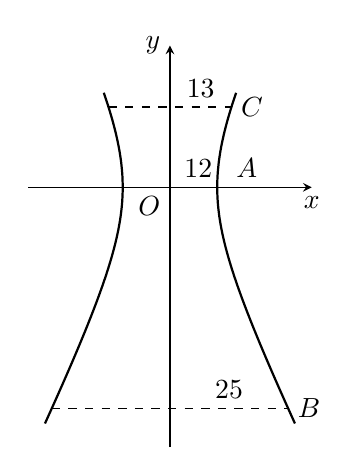
\begin{tikzpicture}[>=stealth, scale=.6]
\draw[->](-3,0)--(3,0)node[below]{$x$};
\draw[->](0,-5.5)--(0,3)node[left]{$y$};
\node[below left]{$O$};
\draw[domain=2:-5, smooth, thick]plot({sqrt(.24*\x*\x+1)},\x);
\draw[domain=2:-5, smooth, thick]plot({-sqrt(.24*\x*\x+1)},\x);
\draw[dashed](-1.3, 1.7)--(0,1.7)--node[above]{13}(1.3,1.7)node[right]{$C$};
\draw[dashed](-2.5, -4.68)--(0,-4.68)--node[above]{25}(2.5,-4.68)node[right]{$B$};
\draw(0,0)--node[above]{12}(1.2,0)node[above right]{$A$};
\end{tikzpicture}
\end{minipage}
    \caption{}
\end{figure}

\begin{solution}
在图3.32的坐标系中，双曲线有标准方程$\frac{x^2}{a^2}-\frac{y^2}{b^2}=1$. 
点$A$旋转所成的圆半径最小，$a=12$. 下面求$b$.

设$B$是双曲线上位于通风塔下口的一点，它的坐标为
$(25,y_1)$；$C$是双曲线上位于通风塔上口的一点，它的坐标为
$(13,y_2)$. 因为$B$、$C$在双曲线上，所以
\[\frac{25^2}{12^2}-\frac{y^2_1}{b^2}=1,\qquad \frac{13^2}{12^2}-\frac{y^2_2}{b^2}=1\]
解得
\[\begin{split}
    y_1&=-\frac{b}{12}\sqrt{25^2-12^2}=-\frac{b}{12}\sqrt{481}\\
    y_2&=\frac{b}{12}\sqrt{13^2-12^2}=\frac{5}{12}b
\end{split}\]
因为塔高55米，所以$y_2-y_1=55$即
\[\frac{5b}{12}+\frac{b\sqrt{481}}{12}=55\]
解得$b\approx 24.5$（米）．

所以双曲线方程（近似）为$\frac{x^2}{12^2}-\frac{y^2}{24.5^2}=1$
\end{solution}


\begin{example}
    以已知双曲线的虚轴为实轴，实轴为虚轴的双曲线叫做原双曲线的\textbf{共轭双曲线}. 求证：
\begin{enumerate}[(1)]
\item 双曲线和它的共轭双曲线有共同的渐近线；
\item 双曲线和它的共轭双曲线的四个焦点在同一个圆上．
\end{enumerate}
\end{example}

\begin{proof}
\begin{enumerate}[(1)]
\noindent
\begin{minipage}{.48\textwidth}
\item 设已知双曲线的方程是
$$\frac{x^2}{a^2}-\frac{y^2}{b^2}=1$$
根据定义，它的共轭双曲线的方程是
\[\frac{y^2}{b^2}-\frac{x^2}{a^2}=1\]

已知双曲线的渐近线方程是$$y=\pm\frac{b}{a}x$$
它的共轭双曲线的渐近线方程是
\[x=\pm\frac{a}{b}y,\quad \text{即}\quad y=\pm\frac{b}{a}x\]
\end{minipage}
\hfill
\begin{minipage}{.5\textwidth}
\centering
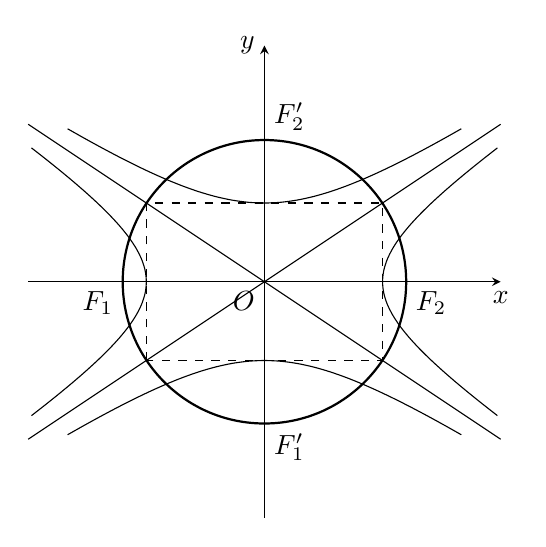
\begin{tikzpicture}[>=stealth]
\draw[->](-3,0)--(3,0)node[below]{$x$};
\draw[->](0,-3)--(0,3)node[left]{$y$};
\node[below left]{$O$};
\draw[domain=-1.7:1.7, smooth]plot({sqrt(2.25*\x*\x+2.25)},\x);
\draw[domain=1.7:-1.7, smooth]plot({-sqrt(2.25*\x*\x+2.25)},\x);

\draw[domain=-2.5:2.5, smooth]plot(\x, {sqrt(.444*\x*\x+1)});
\draw[domain=2.5:-2.5, smooth]plot(\x, {-sqrt(.444*\x*\x+1)});

\draw[domain=-3:3]plot(\x, 2/3*\x);
\draw[domain=-3:3]plot(\x, -2/3*\x);
\draw[thick](0,0)circle(1.8);
\draw[dashed](-1.5,-1)rectangle (1.5,1);
\node at (1.8,0)[below right]{$F_2$};
\node at (0,1.8)[above right]{$F'_2$};
\node at (-1.8,0)[below left]{$F_1$};
\node at (0,-1.8)[below right]{$F'_1$};
\tkzDefPoints{1.8/0/A, 0/1.8/B, -1.8/0/C, 0/-1.8/D}
\tkzDrawPoints(A,B,C,D)
\end{tikzpicture}
\captionof{figure}{}
\end{minipage}
所以双曲线和它的共轭双曲线有共同的渐近线.

\item 设已知双曲线的焦点为$F_1(-c,0)$、$F_2(c,0)$，它的共轭双曲线的焦点为$F'_1(0,-c')$, $F'_2(0,c')$.

$\because\quad c=\sqrt{a^2+b^2},\quad c'=\sqrt{b^2+a^2}$

$\therefore\quad c=c'$

所以四个焦点$F_1,F_2,F'_1,F'_2$在同一个圆$x^2+y^2=a^2+b^2$（图3.33）.
\end{enumerate}
\end{proof}

\begin{remark}
\begin{enumerate}[(1)]
    \item  双曲线$\frac{x^2}{a^2}-\frac{y^2}{b^2}=1$的共轭双曲线是$\frac{x^2}{a^2}-\frac{y^2}{b^2}=-1$，它们有共同的渐近线$\frac{x^2}{a^2}-\frac{y^2}{b^2}=0$，即$\frac{x}{a}\pm \frac{y}{b}=0$.
    
    可以证明：以直线$\frac{x}{a}\pm \frac{y}{b}=0$为渐近线的双曲线方程是$\frac{x^2}{a^2}-\frac{y^2}{b^2}=\lambda$ （$\lambda$是参数）.
 \item 双曲线$\frac{x^2}{a^2}-\frac{y^2}{b^2}=1$与双曲线$\frac{y^2}{a^2}-\frac{x^2}{b^2}=1$都没有共同的
    渐近线($a\ne b$).
\end{enumerate}
\end{remark}    

\begin{example}
    求与双曲线$\frac{x^2}{9}-\frac{y^2}{16}=1$有共同的渐近线，且经过点$A(-3,2\sqrt{3})$的双曲线方程.
\end{example}

\begin{solution}
    设与双曲线$\frac{x^2}{9}-\frac{y^2}{16}=1$有共同的渐近线的双曲线方程为$\frac{x^2}{9}-\frac{y^2}{16}=\lambda$

    $\because\quad $它过点$A(-3,2\sqrt{3})$

$\therefore\quad \lambda=\frac{(-3)^2}{9}-\frac{(2\sqrt{3})^2}{16}=1-\frac{3}{4}=\frac{1}{4}$.

$\therefore\quad$所求双曲线方程为$\frac{x^2}{9}-\frac{y^2}{16}=\frac{1}{4}$，即
$\frac{x^2}{\frac{9}{4}}-\frac{y^2}{4}=1$.
\end{solution}

\noindent
\begin{minipage}{.52\textwidth}\CTEXindent
联想椭圆的几何性质，我们会想到下面的问题：

双曲线$\frac{y^2}{a^2}-\frac{x^2}{b^2}=1$上任意一点$P(x,y)$到其一个焦点$F(c,0)$与对应的直线$\ell:\; x=\frac{a^2}{c}$的距离比是否也是常数$e=\frac{c}{a}$?（图3.34）

作$PE\bot\ell$于$E$，则$|PE|$为点$P$到直线$\ell$的距离，$|PE|=\left|x-\frac{a^2}{c}\right|$.

$\therefore\quad \frac{|PF|}{|PE|}=\frac{\sqrt{(x-c)^2+y^2}}{\left|x-\frac{a^2}{c}\right|}$.
\end{minipage}
\hfill
\begin{minipage}{.45\textwidth}
\centering
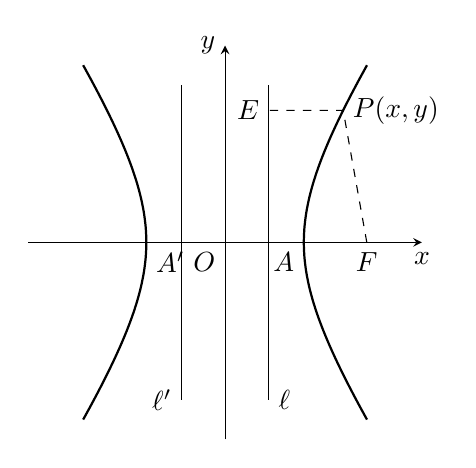
\begin{tikzpicture}[>=stealth]
\draw[->](-2.5,0)--(2.5,0)node[below]{$x$};
\draw[->](0,-2.5)--(0,2.5)node[left]{$y$};
\node[below left]{$O$};
\draw[domain=-2.25:2.25, smooth, thick]plot({sqrt(.444*\x*\x+1)},\x);
\draw[domain=2.25:-2.25, smooth, thick]plot({-sqrt(.444*\x*\x+1)},\x);
\draw(-.556,-2)node[left]{$\ell'$}--(-.556,2);
\draw(.556,-2)node[right]{$\ell$}--(.556,2);
\draw[dashed](1.8,0)node[below]{$F$}--(1.5,1.677)node[right]{$P(x,y)$}--(.556,1.677)node[left]{$E$};
\tkzDefPoints{1.8/0/F, -1.8/0/F'}
\tkzDrawPoints(F,F')
\tkzLabelPoints[below](F')
\tkzDefPoints{.556/0/A, .556/1.667/B, 1.5/1.667/C}
\tkzMarkRightAngles[size=.2](A,B,C)
\node at (1,0)[below left]{$A$};
\node at (-1,0)[below right]{$A'$};
\end{tikzpicture}
\captionof{figure}{}
\end{minipage}

$\because\quad$点$P$在双曲线上，

$\therefore\quad y^2=\frac{b^2}{a^2}(x^2-a^2)=\frac{c^2-a^2}{a^2}(x^2-a^2)$

\[\begin{split}
    \frac{|PF|}{|PE|}&=\frac{\sqrt{(x-c)^2+\frac{c^2-a^2}{a^2}(x^2-a^2)}}{\left|x-\frac{a^2}{c}\right|}=\frac{\sqrt{\left(\frac{c}{a}x\right)^2-2cx+a^2}}{\left|x-\frac{a^2}{c}\right|}\\
    &=\frac{\sqrt{\left(\frac{c}{a}x-a\right)^2}}{\left|x-\frac{a^2}{c}\right|}=\frac{\frac{c}{a}\left|x-\frac{a^2}{c}\right|}{\left|x-\frac{a^2}{c}\right|}=e
\end{split}\]

$\therefore\quad \frac{|PF|}{|PE|}=e$

还可以证明，具有上述性质的点的轨迹是双曲线. 因此双曲线还可以如下定义.

\begin{thm}
   {定义} 平面内，到一个定点$F$的距离与到一条定直线的距离的比是常数$e=\frac{c}{a}\; (e>1)$的点的轨迹叫做双曲线. 这个定点$F$叫做双曲线的焦点，这条直线$\ell$叫做双曲线的准线，常数$e$叫做双曲线的离心率. 
\end{thm}

可以证明，对于双曲线$\frac{x^2}{a^2}-\frac{y^2}{b^2}=1$，相应于焦点$F(c,0)$的准线是直线$x=\frac{a^2}{c}$；相应于焦点$F(-c,0)$的准线是直线$x=-\frac{a^2}{c}$.

\begin{example}
过双曲线$\frac{x^2}{a^2}-\frac{y^2}{b^2}=1$的右焦点$F(c,0)$作其一条渐近线$y=\frac{b}{a}x$的垂线，垂足为$M$，过$M$作直线$\ell\bot x$轴，求直线$\ell$的方程（如图3.35）．

\end{example}

\begin{solution}
过点$F(c,0)$与直线$y=\frac{b}{a}x$垂直的直线方程是$y=-\frac{a}{b}(x-c)$

\noindent
\begin{minipage}{.35\textwidth}
\[\begin{cases}
    y=\frac{b}{a}x\\[1.5ex]
    y=-\frac{a}{b}(x-c)
\end{cases}\]
\[\begin{split}
    \frac{b}{a} x&=-\frac{a}{b}(x-c)\\
    \frac{b^2+a^2}{ab}x&=\frac{ac}{b}\\
    \frac{c^2}{ab}x&=\frac{ac}{b}\\
    x&=\frac{a^2}{c}
\end{split}\]
\end{minipage}
\hfill
\begin{minipage}{.6\textwidth}
\centering
\begin{tikzpicture}[>=stealth, scale=.85]
\draw[->](-4,0)--(4,0)node[below]{$x$};
\draw[->](0,-3)--(0,3)node[left]{$y$};
\node[below left]{$O$};
\draw[domain=-2.5:2.5, smooth, thick]plot({sqrt(1.23*\x*\x+1)},\x);
\draw[domain=-2.5:2.5, smooth, thick]plot({-sqrt(1.23*\x*\x+1)},\x);
\draw[domain=-3:3]plot(\x, 0.9*\x);
\draw[domain=-3:3]plot(\x, -0.9*\x);
\tkzDefPoints{1.35/0/F}
\draw(.74,2.5)--(.74,-2.5)node[right]{$\ell$};
\tkzLabelPoints[below](F)
\draw[thick](.74,.669)node[left]{$M$}--(F);


\end{tikzpicture}
\captionof{figure}{}
\end{minipage}


$\because\quad $点$M$的横坐标为$\frac{a^2}{c}$，$\ell\bot x$轴

$\therefore\quad $直线$\ell$的方程是$x=\frac{a^2}{c}$.
\end{solution}

\subsection*{3.12 练习}
\begin{enumerate}
  

    \item 求下列双曲线的实轴和虚轴的长、顶点和焦点坐标、离心率、渐近线方程和准线方程：
\begin{multicols}{2}
    \begin{enumerate}[(1)]
\item $x^2-8y^2=32$;
\item $9x^2-y^2=81$;
\item $x^2-y^2=-4$;
\item $\frac{x^2}{49}-\frac{y^2}{25}=-1$.     
    \end{enumerate}
\end{multicols}

\item 求适合下列条件的双曲线的标准方程：
\begin{enumerate}[(1)]
    \item 顶点在$x$轴上，两顶点的距离是8，$e=\frac{5}{4}$;
    \item 焦点在$y$轴上，焦距是16，$e=\frac{4}{3}$.
\end{enumerate}

\item 双曲线的中心在原点，焦点在坐标轴上，一条渐近线为直线$3x+5y=0$，求离心率$e$.
\item 等轴双曲线的一个焦点是$F(-6,0)$，求它的标准方程和渐近线方程.
\item 填空：
\begin{enumerate}[(1)]
    \item 以双曲线$\frac{x^2}{16}-\frac{y^2}{9}=1$的焦点为顶点，顶点为焦点的椭圆方程为\blank\blank.
    \item 若双曲线$\frac{x^2}{64}-\frac{y^2}{36}=1$上一点$P$到它的右焦点的距离是8，则点$P$到相应的右准线的距离是\blank\blank.
    \item 若点$P$在双曲线$\frac{x^2}{9}-\frac{y^2}{16}=1$上，且$|PF_1|+|PF_2|=
    26$ （$F_1$、$F_2$为焦点），则$\cos\angle F_1PF_2=\blank\blank$.
    \item 若双曲线及其共轭双曲线的离心率分别为$e_1$、$e_2$，则$\frac{1}{e^2_1}+\frac{1}{e^2_2}=\blank\blank$.
\end{enumerate}
\end{enumerate}

\section{双曲线的参数方程}
从不同的角度考虑，可得到其不同的参数方程.如把方程做如下的变形：
\[\frac{x^2}{a^2}-\frac{y^2}{b^2}=1  \quad \Rightarrow \quad \left(\frac{x}{a}\right)^2-\left(\frac{y}{b}\right)^2=1\]
这后一方程的结构特征容易使我们联想到$\sec^2\theta-\tan^2\theta=1$，从而设

\noindent
\begin{minipage}{.47\textwidth}\CTEXindent
    \begin{equation}
        \begin{cases}
        \frac{x}{a}=\sec\theta \\[1.5ex]
        \frac{y}{b}=\tan\theta
    \end{cases}\Rightarrow \begin{cases}
        x=a\sec\theta\\
        y=b\tan\theta
    \end{cases}\tag{1}
    \end{equation}
        
    以参数方程(1)的结构特征为线索可以构造出图3.36．由此我们可以看出参数$\theta$的几何意义和取值范围（图中大圆半径为$a$，小圆半径为$b$，$A'A, BB'$分别是两圆的切线，$PA'\bot x$轴，$PB'\parallel x$轴）$\theta$称为$P(x,y)$的\textbf{离心角}，(1)称为双曲线的\textbf{离心角式参数方程}.

    若把方程变为
\end{minipage}
\hfill
\begin{minipage}{.5\textwidth}
\centering
\begin{tikzpicture}[>=stealth, scale=.9]
\draw[->](-3,0)--(4,0)node[below]{$x$};
\draw[->](0,-3)--(0,3)node[left]{$y$};
\node[below left]{$O$};
\draw[domain=-1.9:1.9, smooth]plot({sqrt(2.25*\x*\x+2.25)},\x);
\draw[domain=1.7:-1.7, smooth]plot({-sqrt(2.25*\x*\x+2.25)},\x);
\draw[domain=-3:3.5]plot(\x, 2/3*\x);
\draw[domain=-3:3.5]plot(\x, -2/3*\x);
\draw[dashed](0,0)circle(1.5);
\draw[dashed](0,0)circle(1);
\draw[thick](-1.5,-1)rectangle (1.5,1);
\tkzDefPoint(60:1.5){A}
\tkzDefPoint(60:1){A1}
\tkzDefPoint(60:2){B'}
\tkzDefPoints{3/0/A', 0/0/O, 1/0/B}
\tkzDrawSegments[dashed](O,B' A,A' B,B')

\tkzLabelPoints[above](A,B')
\tkzLabelPoints[below](A',B)

\draw(.5,0) arc (0:60:.5)node[right]{$\theta$};
\draw[dashed](B')--+(2,0)node[below right]{$P(x,y)$}--(A');
\end{tikzpicture}
\captionof{figure}{}
\end{minipage}

\[\left(\frac{x}{a}\right)^2-\left(\frac{y}{b}\right)^2=1\quad \Rightarrow\quad \left(\frac{x}{a}+\frac{y}{b}\right)\left(\frac{x}{a}-\frac{y}{b}\right)=1\]
后者却容易使我们联想到$\tan\theta\cdot \cot\theta =1$，从而设
\begin{align}
    \begin{cases}
    \frac{x}{a}+\frac{y}{b}=\tan\theta\\[1.5ex]
    \frac{x}{a}-\frac{y}{b}=\cot\theta
\end{cases}&\Rightarrow \begin{cases}
    x=\frac{a}{2}\left(\tan\theta+\cot\theta\right)\\[1.5ex]
    y=\frac{b}{2}\left(\tan\theta-\cot\theta\right)
\end{cases}\nonumber \\
&\xRightarrow{\text{令}t=\tan\theta} \begin{cases}
    x=\frac{a}{2}\left(t+\frac{1}{t}\right)\\[1.5ex]
    y=\frac{b}{2}\left(t-\frac{1}{t}\right)
\end{cases}\tag{2}
\end{align}



\begin{example}
    已知双曲线$x^2-\frac{y^2}{4}=1$和点$A(0,1)$，求双曲线上与点$A$距离最近的点$Q$到点$A$的距离.
\end{example}

\begin{solution}
由条件可得双曲线的参数方程
\[\begin{cases}
    x=\sec\alpha\\
    y=2\tan\alpha
\end{cases}\text{（$\alpha$为参数）}\]
则设双曲线上动点$P$的坐标为$(\sec\alpha, 2\tan\alpha)$，
\[\begin{split}
 |PA|^2=\sec^2\alpha+(2\tan\alpha-1)^2
&=\sec^2\alpha+4\tan^2\alpha-4\tan\alpha+1\\
&=5\tan^2\alpha-4\tan\alpha+2\\
&=5\left(\tan\alpha-\frac{2}{5}\right)+\frac{6}{5}   
\end{split}\]

$\therefore\quad$当$\tan\alpha=\frac{2}{5}$时，$|PA|_{\min}=\frac{\sqrt{30}}{5}$.

此时，$x=\sec\alpha=\pm\sqrt{\tan^2\alpha+1}=\pm\frac{\sqrt{29}}{5}$, $y=2\tan\alpha=\frac{4}{5}$，所以双曲线上与点$A$距离最近的点为点$\left(\pm\frac{\sqrt{29}}{5},\; \frac{4}{5}\right)$.
\end{solution}


\begin{example}
    已知双曲线$\frac{x^2}{a^2}-\frac{y^2}{b^2}=1$上动点$P$，求线段$OP$的定比分点$M$的轨迹，其中$\lambda=\frac{OM}{MP}=2$.
\end{example}

\begin{solution}
由双曲线$\frac{x^2}{a^2}-\frac{y^2}{b^2}=1$的参数方程
\[\begin{cases}
    x=a\sec\alpha\\ y=b\tan\alpha
\end{cases}\]
设点$P$坐标为$(a\sec\alpha,b\tan\alpha)$，则$M(x,y)$有
\[\begin{cases}
    x=\frac{2a\sec\alpha}{3} \\[1.5ex]
    y=\frac{2b\tan\alpha}{3} 
\end{cases}\]
此方程组即是点$M$的轨迹的参数方程，消参得点$M$的轨迹的普通方程
\[\frac{x^2}{\frac{4a^2}{9}}-\frac{y^2}{\frac{4b^2}{9}}=1\]
$\therefore\quad M$的轨迹是双曲线$\frac{x^2}{\frac{4a^2}{9}}-\frac{y^2}{\frac{4b^2}{9}}=1$.
\end{solution}

\subsection*{3.13 练习}
\begin{enumerate}
    \item 求证：等轴双曲线$x^2-y^2=a^2\; (a>0)$上任一点$P$到其两个焦点$F_1,F_2$的距离之积，等于点$P$到其中心的距离的平方.
    \item 已知参数方程$\begin{cases}
        x=\left(t+\frac{1}{t}\right)\sin\theta\\[1.5ex]
        y=\left(t-\frac{1}{t}\right)\cos\theta\\
    \end{cases}$
\begin{enumerate}[(1)]
    \item 若$t$为常数，$\theta$为参数，方程表示什么曲线？
    \item 若$t$为参数，$\theta$为常数，方程表示什么曲线？
\end{enumerate}
\end{enumerate}

\section{双曲线与直线的位置关系}
由于双曲线不是封闭曲线，因此，一条直线与双曲线的位置与直线与椭圆的位置关系相比会有所不同. 

\begin{example}
    试确定直线$y=k(x-1)\; (k\in\R)$与双曲线$x^2-y^2=4$的公共点的个数．
\end{example}

\begin{analyze}
    我们先在同一坐标系中作出双曲线$x^2-y^2=4$及动直线$y=k(x-1)\; (k\in\R)$，观察可能出现的各种情况，然后解方程组，进行对照.
\end{analyze}

\begin{solution}

\noindent
\begin{minipage}{.43\textwidth}\CTEXindent
\[\begin{cases}
    y=k(x-1) &(1)\\
    x^2-y^2=4&(2)
\end{cases}\]
(1)代入(2)，得
\[\begin{split}
    x^2-k^2(x-1)^2&=4\\
(1-k^2)x^2+2k^2x-(k^2+4)&=0
\end{split}\]

当$1-k^2=0$即$k=\pm 1$时，方程变为$2x-5=0$, 
$x=\frac{5}{2}$.
\end{minipage}
\hfill
\begin{minipage}{.55\textwidth}
\centering
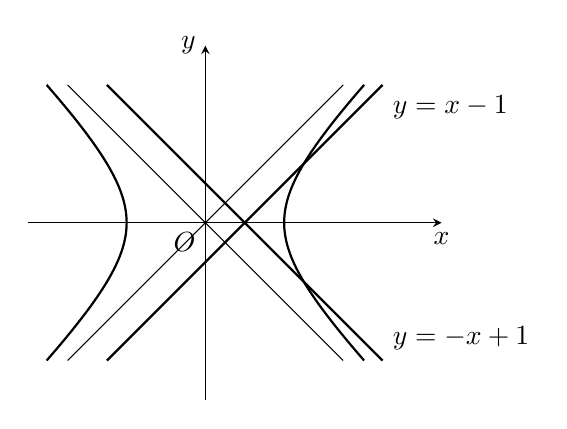
\begin{tikzpicture}[>=stealth, scale=.5]
\draw[->](-4.5,0)--(6,0)node[below]{$x$};
\draw[->](0,-4.5)--(0,4.5)node[left]{$y$};
\node[below left]{$O$};
\draw[domain=-3.5:3.5, smooth, thick]plot({sqrt(\x*\x+4)},\x);
\draw[domain=-3.5:3.5, smooth, thick]plot({-sqrt(\x*\x+4)},\x);
\draw[domain=-3.5:3.5]plot(\x, \x);
\draw[domain=-3.5:3.5]plot(\x, -\x);
\draw[domain=-2.5:4.5, thick]plot(\x, \x-1)node[below right]{$y=x-1$};
\draw[domain=-2.5:4.5, thick]plot(\x, -\x+1)node[above right]{$y=-x+1$};
\end{tikzpicture}
\captionof{figure}{}
\end{minipage}


这就是说，当$k=\pm 1$时，直线$y=\pm (x-1)$恰与双曲线$x^2-y^2=4$的渐近线$y=\pm x$平行，直线与双曲线右支的一个
交点的横坐标为$x=\frac{5}{2}$（如图3.37）．

当$1-k\ne 0$即$k\ne \pm1$时，
方程
$(1-k)x^2+2k^2x-(k^2+4)=0$是二次方程.
\[\Delta =4[k^4+(1-k^2)(k^2+4)]=4(4-3k^2)\]

当$\begin{cases}
    4-3k^2>0\\ k\ne \pm 1
\end{cases}$，即$k\in\left(-\frac{2\sqrt{3}}{3},\; -1\right)\cup(-1,1)\cup\left(1,\;\frac{2\sqrt{3}}{3}\right)$时，$\Delta >0$，方
程组有两组不等的实根. 这时直线$y=k(x-1)$与双曲线$x^2-y^2=4$有两个不同的交点. 其中，当$-1<k<1$时，直线与双曲线的两支
各有一个交点，当$-\frac{2\sqrt{3}}{3}<k<-1$或$1<k<\frac{2\sqrt{3}}{3}$时，直线与双曲线的右支有两个交点.

当$4-3k^2=0$即$k=\pm\frac{2\sqrt{3}}{3}$时，$\Delta=0$，方程组有两组相等当的实根. 这时直线$y=k(x-1)$与双曲线$x^2-y^2=4$只有一个公共点（称直线与双曲线相切）.

当$4-3k^2<0$即$k\in\left(-\infty,\; -\frac{2\sqrt{3}}{3}\right)\cup\left(\frac{2\sqrt{3}}{3},\;+\infty\right)$时，$\Delta<0$，方程组无实数解. 这时直线$y=k(x-1)$与双曲线$x^2-y^2=4$没有公共点.
\end{solution}

\begin{remark}
\begin{enumerate}[(1)]
    \item 当直线与双曲线有两个交点时，称此直线与双曲线相交，两个交点之间的部分又称为双曲线的弦.
    \item 读者还可过点$A(2,0)$或$B(3,0)$作直线，就直线的各种位置确定它们与双曲线$x^2-y^2=4$的位置关系.
\end{enumerate}
\end{remark}

\begin{example}
求证：任一直线$\ell$截双曲线及其渐近线所得双曲线与渐近线之间的线段相等.
\end{example}

\begin{analyze}
如图3.38，如果我们老老实实计算线段$AC$和$BD$的长度，看看它们的值是否相等，这是一件十分困难的事. 不妨换个角度想，如果能证出线段$AB$与$CD$的中点彼此重合，就能保证
$|AC|=|BD|$.
\end{analyze}

\begin{proof}
\textbf{解法1：}设双曲线的方
程为
\begin{equation}
    \frac{x^2}{a^2}-\frac{y^2}{b^2}=1\tag{1}
\end{equation}
则其渐近线的方程为
\begin{equation}
    \frac{x^2}{a^2}-\frac{y^2}{b^2}=0 \tag{2}
\end{equation}
\begin{enumerate}[(1)]
\item 若直线$\ell\bot x$轴，由双曲线关于$x$轴的对称性，显然命题成立.
\item 若直线$\ell$与$x$轴不垂直．设$\ell$的方程为$y=kx+m$，且$\ell$与双曲线交于$A$、$B$两点；$\ell$与其渐近线交于$C$、$D$两点. 
\end{enumerate}
\[\begin{cases}
    y=kx+m\\ b^2x^2-a^2y^2=a^2b^2
\end{cases}\]
得$(b^2-a^2k^2)x^2-2a^2mkx-a^2(m^2+b^2)=0$.

$\therefore\quad $线段$AB$中点$M$的横坐标为
\begin{equation}
    x_M=\frac{x_A+x_B}{2}=\frac{a^2mk}{b^2-a^2k^2} \tag{3}
\end{equation}
\[\begin{cases}
    y=kx+m\\ b^2x^2-a^2y^2=a^2b^2
\end{cases}\]
得$(b^2-a^2k^2)x^2-2a^2mkx-a^2m^2=0$.

\noindent
\begin{minipage}{.45\textwidth}\CTEXindent
$\therefore\quad$线段$CD$中点$M'$的横坐标为
\begin{equation}
    x_{M'}=\frac{x_C+x_D}{2}=\frac{a^2mk}{b^2-a^2k^2}  \tag{4}
\end{equation}

由(3)、(4)得$x_M=x_{M'}$.

又$\because\quad M,M'\in\ell$

$\therefore\quad $点$M$与$M'$重合

$\because\quad \begin{cases}
    |AM|=|MB|\\|CM|=|MD|
\end{cases}$

$\therefore\quad |AC|=|DB|$
\end{minipage}
\hfill
\begin{minipage}{.52\textwidth}
\centering
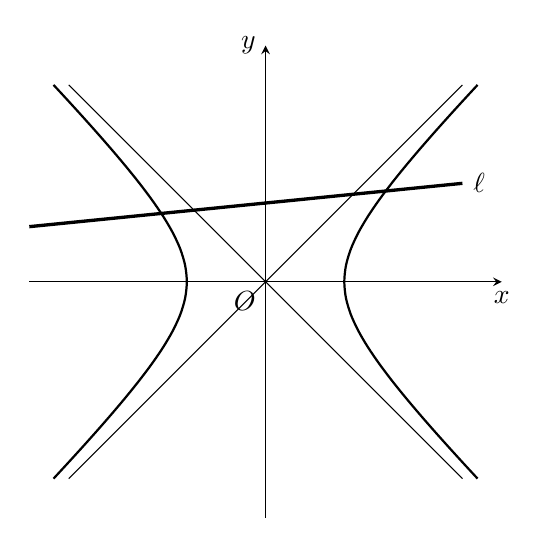
\begin{tikzpicture}[>=stealth]
\draw[->](-3,0)--(3,0)node[below]{$x$};
\draw[->](0,-3)--(0,3)node[left]{$y$};
\node[below left]{$O$};
\draw[domain=-2.5:2.5, smooth, thick]plot({sqrt(\x*\x+1)},\x);
\draw[domain=-2.5:2.5, smooth, thick]plot({-sqrt(\x*\x+1)},\x);
\draw[domain=-2.5:2.5]plot(\x, \x);
\draw[domain=-2.5:2.5]plot(\x, -\x);

\draw[domain=-3:2.5, very thick]plot(\x, .1*\x+1)node[right]{$\ell$};
\tkzDefPoints{1.11/1.11/D, -.909/.909/C, 0.1/1.01/M}
\tkzLabelPoints[above](C,D,M)
\tkzDrawPoints(M,C,D)
\tkzDefPoints{1.53/1.15/B, -1.324/.87/A}
\tkzLabelPoints[below](A,B)
\tkzDrawPoints(A,B)

\end{tikzpicture}
\captionof{figure}{}
\end{minipage}

\textbf{解法2：}当直线$\ell$与$x$轴不垂直时，设直线$y=kx+m$与双曲线$\frac{x^2}{a^2}-\frac{y^2}{b^2}=1$交于$A(x_1,y_1)$、$B(x_2,y_2)$点，与其渐近线$\frac{x^2}{a^2}-\frac{y^2}{b^2}=0$交于$C(x_3,y_3)$、$D(x_4,y_4)$点. $AB$的中点为$M$，$CD$的中点为$M'$. 则
\[\begin{cases}
    \frac{x^2_1}{a^2}-\frac{y^2_1}{b^2}=1&(1)\\[1.5ex]
    \frac{x^2_2}{a^2}-\frac{y^2_2}{b^2}=1&(2)\\[1.5ex]
    y_2-y_1=k(x_2-x_1) &(3)\\
    x_1+x_2=2x_M &(4)\\
    y_1+y_2=2y_M &(5)\\
    y_M=kx_M+m &(6)
\end{cases}\]
$(2)-(1)$得
\[\begin{split}
    \frac{x^2_2-x^2_1}{a^2}&=\frac{y^2_2-y^2_1}{b^2}\\
    \frac{(x_2-x_1)(x_2+x_1)}{a^2}&=\frac{(y_2-y_1)(y_2+y_1)}{b^2}
\end{split}\]
将(3)(4)(5)代入，得
\[\begin{split}
    \frac{x_M}{a^2}&=\frac{ky_M}{b^2}\\
    b^2x_M&=ka^2 y_M=ka^2(kx_M+m)\\
\end{split}\]

$\therefore\quad x_M=\frac{kma^2}{b^2-k^2a^2}$

同理可求：$x_{M'}=\frac{kma^2}{b^2-k^2a^2}$

$\therefore\quad AB$与$CD$的中点重合.

$\therefore\quad |AC|=|DB|$.
\end{proof}

\begin{example}
    给定双曲线$C:\; x^2-\frac{1}{2}y^2=1$，过点$B(1,1)$能否作直线$m$，使与双曲线$C$交于两点$Q_1$、$Q_2$，且使点$B$平分线段$Q_1,Q_2$. 这样的$m$如果存在，求出其方程，若不存在，说明理由.
\end{example}

\begin{analyze}
    此题是属于存在性问题. 解这样的问题可先假设符合条件的直线$m$存在，根据已知条件看能否求出直线的斜率？
\end{analyze}

\begin{solution}
设直线$m$的斜率为$k$，直线$m$与双曲线$x^2-\frac{1}{2}y^2=1$交于$P(x_1,y_1)$, $Q(x_2,y_2)$，且点$B(1,1)$恰好为$PQ$的中点. 则  
\[\begin{cases}
    x^2_1-\frac{1}{2}y_1^2=1&   (1)\\[1.5ex]
    x^2_2-\frac{1}{2}y^2_2=1&   (2)\\[1.5ex]
x_1+x_2=2&  (3)\\
y_1+y_2=2&  (4)\\[1.5ex]
\frac{y_2-y_1}{x_2-x_1}=k&  (5)
\end{cases}\]
$(2)-(1)$得
\[\begin{split}
   x^2_2-x^2_1&=\frac{1}{2}(y^2_2-y^2_1)\\
   (x_2-x_1)(x_2+x_1)&=\frac{1}{2}(y_2-y_1)(y_2+y_1)
\end{split}\]
将(3)(4)代入，得
\[\begin{split}
    2(x_2-x_1) &=(y_2-y_1)\\
    k&=\frac{y_2-y_1}{x_2-x_1}=2
\end{split}\]

$\therefore\quad$直线$m$的方程应为$y-1=2(x-1)$，即$y=2x-1$.

检验$\begin{cases}
    y=2x-1\\[1.5ex] x^2-\frac{1}{2}y^2=1
\end{cases}$
消去$y$得
\[\begin{split}
x^2-\frac{1}{2}(2x-1)^2&=1\\
2x^2-4x+3&=0    
\end{split}\]

$\because\quad \Delta=16-24<0$，方程无实根，

$\therefore\quad $直线$m$与双曲线$x^2-\frac{1}{2}y^2=1$无公共点，这与假设矛盾.

因此符合题意的直线$m$不存在.
\end{solution}

\begin{remark}
\begin{enumerate}[(1)]
\noindent
\begin{minipage}{.5\textwidth}
\item 当求出直线$m$的斜率$k=2$后，不要以为题目已做完，因为解题时所列条件不包含直线$m$与双曲线相交的条件，故应先画示意图（如图3.39），从直观上看一看此直线是否能与双曲线相交？同时进一步做出准确的判断.
    \item 若设直线$m$的方程为$y-1=k(x-1)$.
\[\begin{cases}
    y=kx-(k-1)\\[1.5ex]
    x^2-\frac{1}{2}y^2=1\\
\end{cases}\]
消去$y$得
\end{minipage}
\hfill
\begin{minipage}{.45\textwidth}
\centering
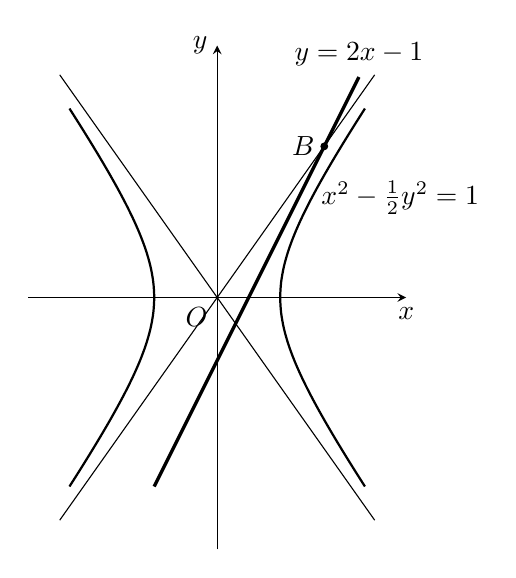
\begin{tikzpicture}[>=stealth, scale=.8]
\draw[->](-3,0)--(3,0)node[below]{$x$};
\draw[->](0,-4)--(0,4)node[left]{$y$};
\node[below left]{$O$};
\draw[domain=-3:3, smooth, thick]plot({sqrt(.5*\x*\x+1)},\x);
\draw[domain=-3:3, smooth, thick]plot({-sqrt(.5*\x*\x+1)},\x);
\draw[domain=-2.5:2.5]plot(\x, 1.414*\x);
\draw[domain=-2.5:2.5]plot(\x, -1.414*\x);
\draw[domain=-1:2.25, very thick]plot(\x, 2*\x-1)node[above]{$y=2x-1$};
\node at (1.5,2)[below right]{$x^2-\frac{1}{2}y^2=1$};
\draw[fill](1.7,2.4)node[left]{$B$}circle(1.5pt);
\end{tikzpicture}
\captionof{figure}{}
\end{minipage}

\[(2-k^2)x^2+2k(k-1)x-(k^2-2k+3)=0\]
所求的$k$应满足
$\begin{cases}
    \Delta >0\\[1.5ex]
    \frac{x_1+x_2}{2}=1
\end{cases}$

这两个条件缺一不可. 它们是使$B$点为直线被双曲线所截弦的中点的充要条件.
\item 读者还可用直线的参数方程试着解此题．
\end{enumerate}
\end{remark}



\subsection*{3.14 练习}
\begin{enumerate}
\item 已知：双曲线的中心在原点，一个焦点为$F(\sqrt{5},0)$，它被直线$y=x-2$截得的弦的中点的横坐标是6，求此双曲线的方程.
\item 已知：双曲线$\frac{x^2}{a^2}-\frac{y^2}{b^2}=1$的左、右两个焦点分别为$F_1$、$F_2$，$AB$是过$F_1$点的双曲线的弦，且$|AB|=m$，求$\triangle ABF_2$的周长.
\item 过双曲线$\frac{x^2}{9}-\frac{y^2}{16}=1$的右焦点$F$作倾斜角为$\frac{\pi}{4}$的弦$AB$，求弦长$|AB|$及中点$C$到$F$的距离.
\end{enumerate}

\section*{习题五}
\begin{center}
    \bfseries A
\end{center}

\begin{enumerate}
    \item  求下列双曲线的实轴和虚轴的长、焦点坐标、焦距、离心率、渐近线方程、准线方程，并画出图形：
\begin{enumerate}[(1)]
    \item $\frac{x^2}{36}-\frac{y^2}{64}=1$
    \item $\frac{y^2}{4}-x^2=1$
    \item $-9{x^2}+{y^2}=81$
    \item $x^2-y^2=4$
\end{enumerate}
    \item  求满足下列条件的双曲线的标准方程：
\begin{enumerate}[(1)]
\item 实轴和虚轴的长分别是12和14，焦点在$x$轴上；
\item 一个焦点的坐标是$(0,-4)$，半虚轴的长是3；
\item 焦距为16，离心率$e=\frac{4}{3}$;
\item 一个焦点为$(10,0)$，和它相应的准线方程是$x=6\frac{2}{5}$;
\item 一条渐近线是$3x-2y=0$，准线方程为$y=4$;
\item 一个焦点是$F_1(-6,0)$且是等轴双曲线.
\end{enumerate}

    \item  求以椭圆$\frac{x^2}{16}+\frac{y^2}{25}=1$的焦点为顶点，而以椭圆的顶点为焦点的双曲线方程.
    \item \begin{enumerate}[(1)]
        \item 求渐近线为$y=\pm\frac{3}{5}x$，且过点$(10,-3\sqrt{3})$的双曲线的标准方程；
        \item 求焦距等于10，且准线间的距离等于6的双曲线的标准方程.
    \end{enumerate}

\item  求与椭圆$x^2+4y^2=64$有共同焦点，且渐近线方程为$x\pm\sqrt{3}y=0$的双曲线的方程.
\item  已知双曲线$16x^2-9y^2=144$.
\begin{enumerate}[(1)]
\item 求此双曲线的焦点坐标、离心率和渐近线方程；
\item 设$F_1$、$F_2$是它的焦点，点$P$在双曲线上，且$|PF_1|\cdot |PF_2|=32$，求$\angle F_2PF_1$的大小.
\end{enumerate}

\item  若直线$\ell$在双曲线$2x^2-3y^2=6$上截得的弦长为4，且$k_{\ell}=2$，求$\ell$的方程．
\item  设$F_1,F_2$为双曲线$\frac{x^2}{4}-y^2=1$的两个焦点，点$P$在双曲线上且$\angle F_1PF_2=90^{\circ}$，求$\triangle F_1PF_2$的面积.
\end{enumerate}

\begin{center}
    \bfseries B
\end{center}

\begin{enumerate}\setcounter{enumi}{8}
    \item 经过双曲线$\frac{x^2}{a^2}-\frac{y^2}{b^2}=1$上的任意一点$P$作两条分别平行干渐近线的直线，求证：这两条直线和两条渐近线所围成的平行四边形的面积为一定值.
    \item 已知双曲线$\frac{y^2}{12}-\frac{x^2}{13}=1$的同一支上有不同的三个点$A(x_1,y_1)$、$B(\sqrt{26},6)$、$C(x_2,y_2)$，它们与焦点$F(0,5)$的距离成等差数列．
\begin{enumerate}[(1)]
    \item 求$y_1+y_2$的值；
    \item 求证线段$AC$的垂直平分线恒过定点，并求出该定点的坐标.
\end{enumerate}
    \item 在相距1400米的$A$、$B$两哨所，听到炮弹爆炸声的时间相差3秒，已知声速是340米/秒，炮弹爆炸点在怎样的曲线上？
    \item 通过双曲线$\frac{x^2}{144}-\frac{y^2}{25}=1$的一个焦点，作$x$轴的垂线，求垂线与双曲线的交点到两焦点的距离.
    \item 证明从双曲线的一个焦点到一条渐近线的距离等于虚半轴长.
    \item 设$P$为双曲线$\frac{x^2}{a^2}-\frac{y^2}{b^2}=1$上任意一点，过$P$作$x$轴的垂线交渐近线于$A$、$B$两点，求证$|PA|\cdot |PB|$为定值.
    \item  求与定点$A(5,0)$及定直线$\ell:\; x=\frac{16}{5}$的距离比是$5:4$的点的轨迹方程.
    \item  $\triangle ABC$一边的两个端点是$B(0,6)$和$C(0,-6)$，另两边斜率的积是$\frac{4}{9}$，求顶点$A$的轨迹.
        \item  若方程$\frac{x^2}{2+m}-\frac{y^2}{1+m}=1$的曲线是双曲线，求$m$的范围.
        \item  当$\alpha$从$0^{\circ}$到$180^{\circ}$变化时，曲线$x^2+y^2\cos\alpha=1$怎样变化？
  
\end{enumerate}

\begin{center}
    \bfseries C
\end{center}

\begin{enumerate}\setcounter{enumi}{18}
    \item  直线$y=ax+1$与双曲线$3x^2-y^2=1$相交于$A$、$B$两点. 是否存在这样的实数$a$，使得点$A$、$B$关于直线$\ell_0:\; y=2x$对称. 如果存在，求出实数$a$，如果不存在说明理由.
\end{enumerate}

\section*{六、抛物线}
\section{抛物线及其标准方程}
我们知道，平面内与一个定点的距离和一条定直线的距离比是常数$e$的点的轨迹，当$e<1$时，是椭圆；当$e>1$时，是双曲线. 那么当$e=1$时，它又是什么曲线呢？

\begin{thm}
   {定义} 平面内与一个定点$F$和一条定直线$\ell$的距离相等（即$e=1$）的点的轨迹叫做\textbf{抛物线}. 点$F$叫做抛物线的\textbf{焦点}，直线$\ell$叫做抛物线的\textbf{准线}.
\end{thm}

为求抛物线的方程，只要抛物线上点的特征性质“代数化”即可.

\noindent
\begin{minipage}{.6\textwidth}\CTEXindent
    取经过焦点$F$且垂直于准线$\ell$的直线为$x$轴，$x$轴与$\ell$相交于点$K$，以线段$KF$的垂直平分线为$y$轴（图3.40）．设$|KF|=P$，那么，焦点$F$的坐标为$\left(\frac{p}{2},0\right)$，准线$\ell$的方程为$x=-\frac{p}{2}$.

    设抛物线上的点$P(x,y)$到$\ell$的距离为$d$. 抛物线也就是集合
    \[P=\left\{\text{点}P\Big||PF|=d \right\}\]
    
    $\therefore\quad \sqrt{\left(x-\frac{p}{2}\right)^2+y^2}=\left|x+\frac{p}{2}\right|$
\end{minipage}
\hfill
\begin{minipage}{.37\textwidth}
\centering
\begin{tikzpicture}[>=stealth, scale=.65]
\draw[->](-2,0)--(5,0)node[below]{$x$};
\draw[->](0,-4.5)--(0,4.5)node[left]{$y$};
\node[below left]{$O$};
\draw[domain=4:-4, very thick, smooth]plot({0.25*\x*\x} , \x);
\tkzDefPoints{1/0/F, 2/2.828/P, -1/0/K, -1/2.828/P'}
\draw(-1,4)node[left]{$\ell$}--(-1,-4);
\tkzMarkRightAngles[size=.2](P,P',K)
\draw[dashed](F)--(P)--(P');
\tkzLabelPoints[below](F)
\tkzLabelPoints[right](P)
\tkzLabelPoints[below left](K)
\tkzDrawPoints(P,F)
\end{tikzpicture}
\captionof{figure}{}
\end{minipage}


将上式两边平方，并化简得
\begin{equation}
    y^2=2px\quad (p>0) \tag{1}
\end{equation}

由于方程变形为同解变形，方程(1)是抛物线的方程.

方程(1)叫做抛物线的标准方程. 它表示的抛物线的焦点在$x$轴的正半轴上，坐标是$\left(\frac{p}{2},0\right)$，它的准线方程是$x=-\frac{p}{2}$.

一条抛物线，由于它在坐标平面上的位置不同，方程也不同. 所以抛物线的标准方程还有其他几种形式：$y^2=-2px$, $x^2=2py$, $x^2=-2py$，它们的焦点坐标，准线方程以及图形列表如下：

\begin{center}
\begin{tabular}{m{3cm}|m{1.8cm}|m{1.5cm}|m{3.5cm}}
\hline
方程& 焦点& 准线& 图形\\
\hline
$y^2=2px\; (p>0)$ & $F\left(\frac{p}{2},\; 0\right)$ & $x=-\frac{p}{2}$ & 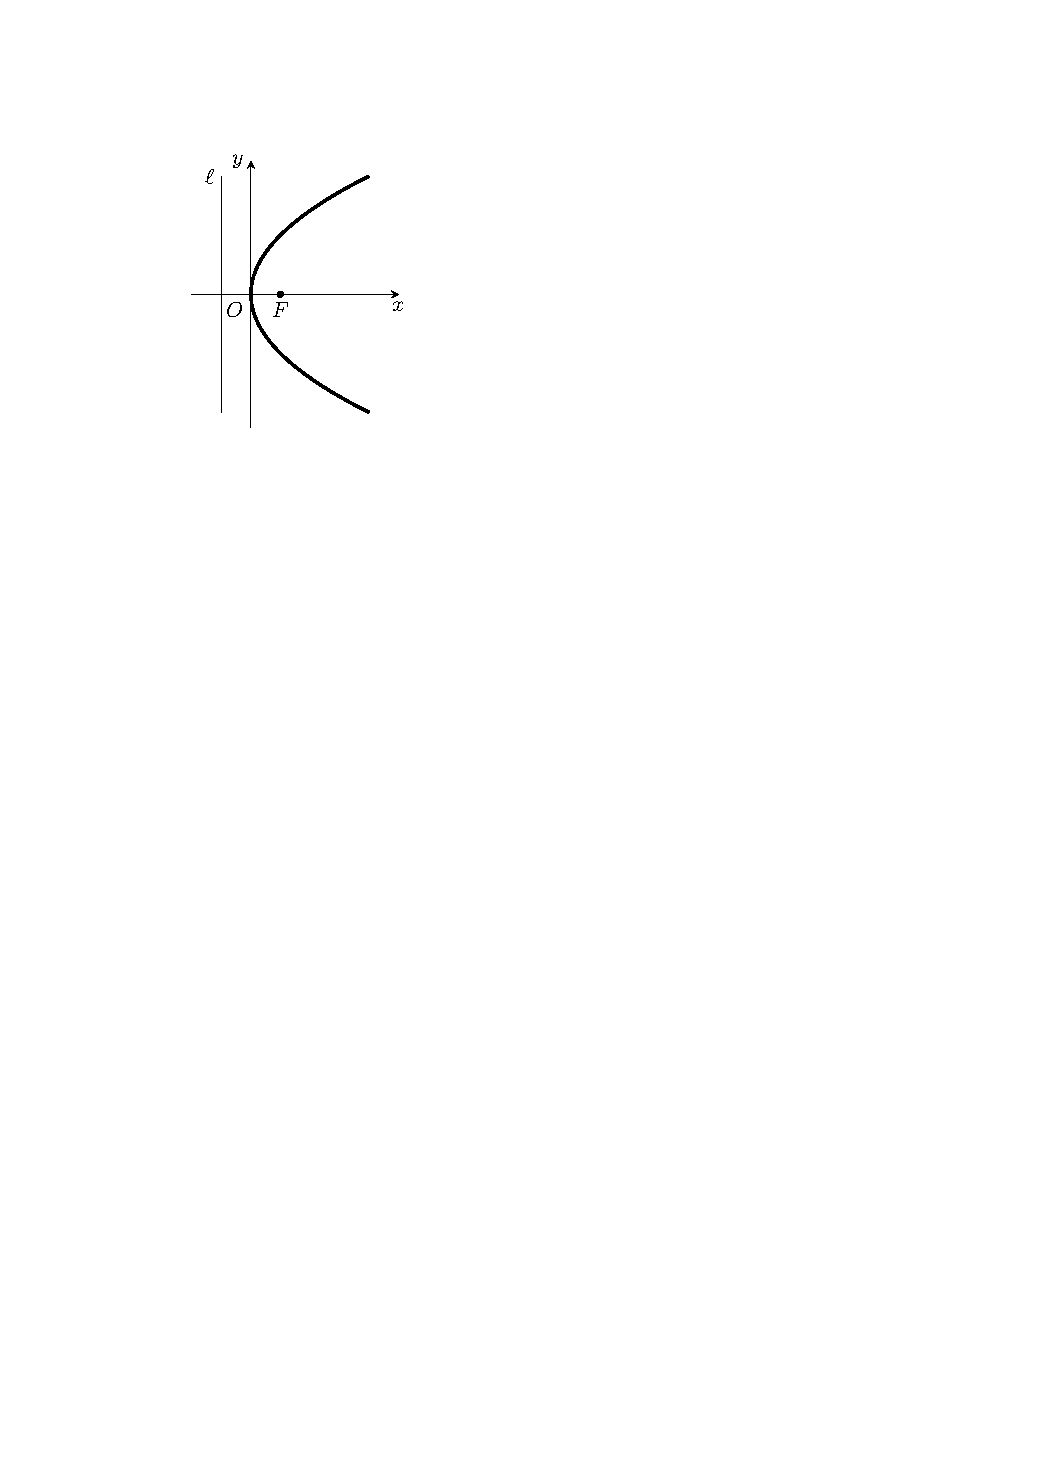
\includegraphics[scale=.7]{fig/para1.pdf} \\\hline
$y^2=-2px\; (p>0)$ & $F\left(-\frac{p}{2},\; 0\right)$ & $x=\frac{p}{2}$ & 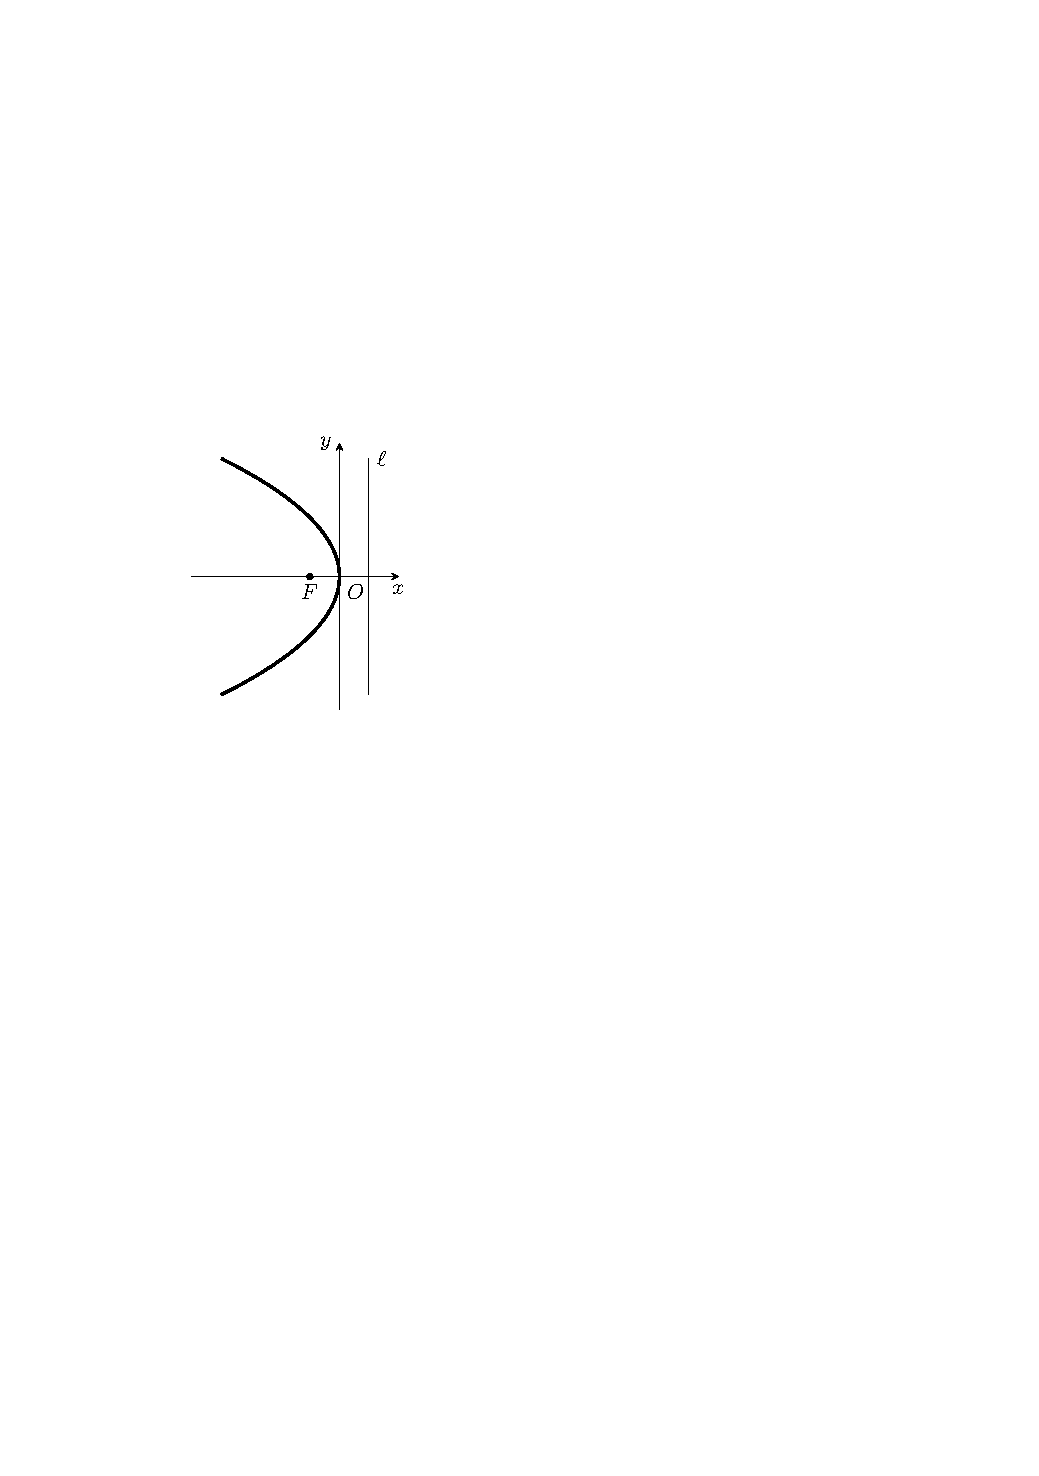
\includegraphics[scale=.7]{fig/para2.pdf} \\\hline
$x^2=2py\; (p>0)$ & $F\left(0,\; \frac{p}{2}\right)$ & $y=-\frac{p}{2}$ & 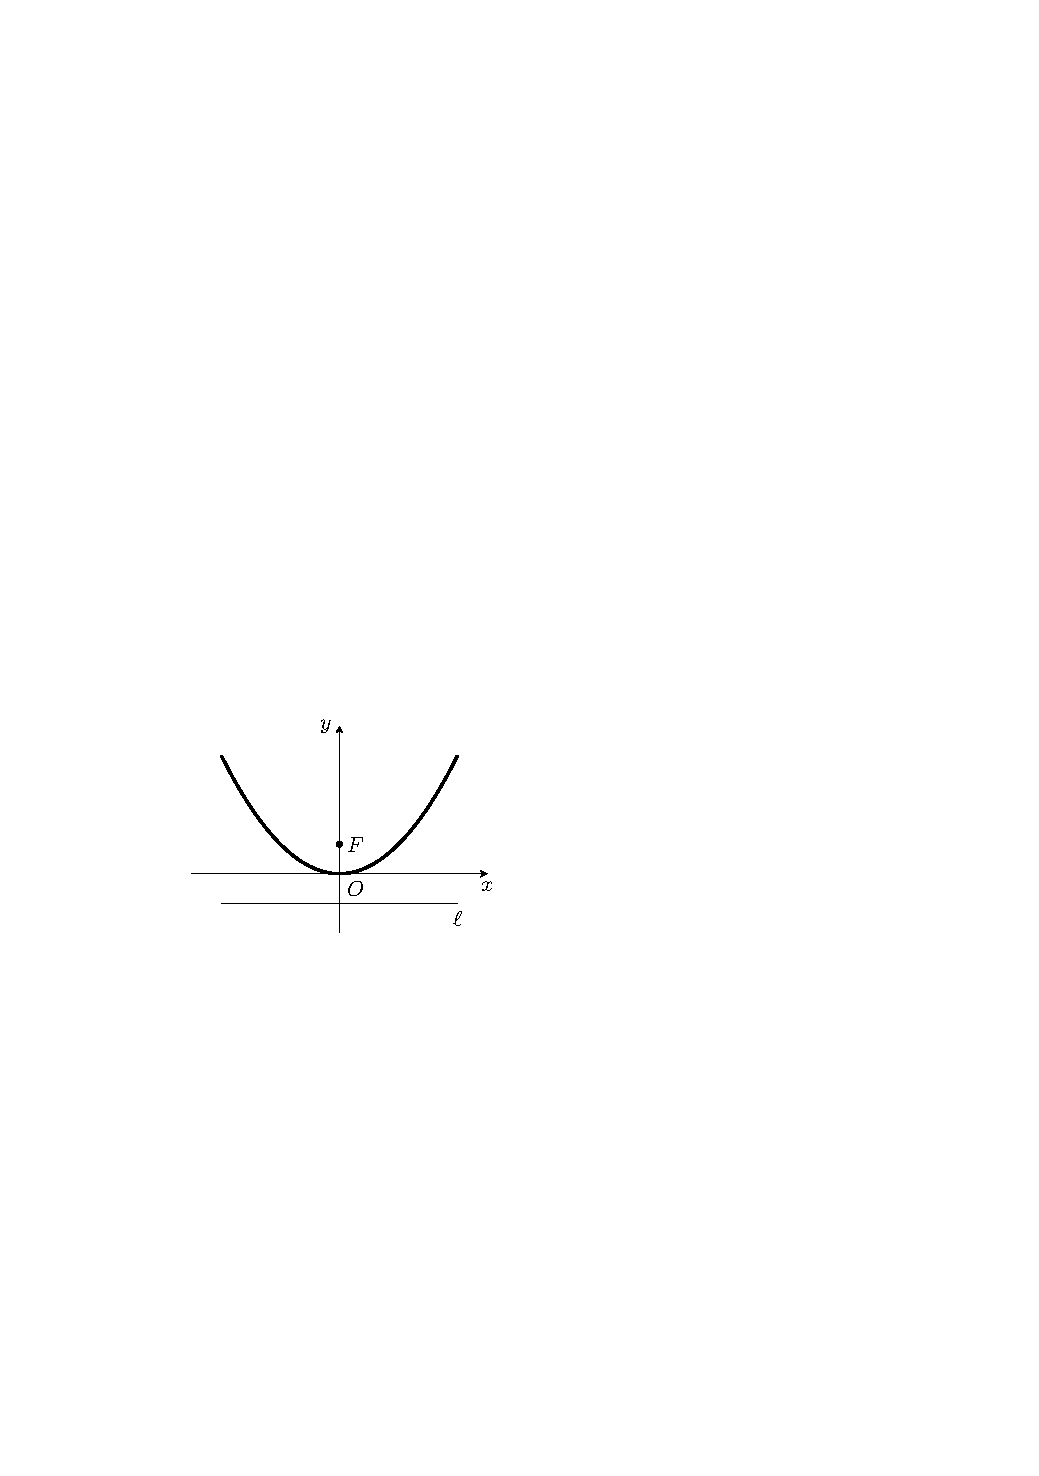
\includegraphics[scale=.7]{fig/para3.pdf} \\\hline
$x^2=-2py\; (p>0)$ & $F\left(0,\; -\frac{p}{2}\right)$ & $y=\frac{p}{2}$ & 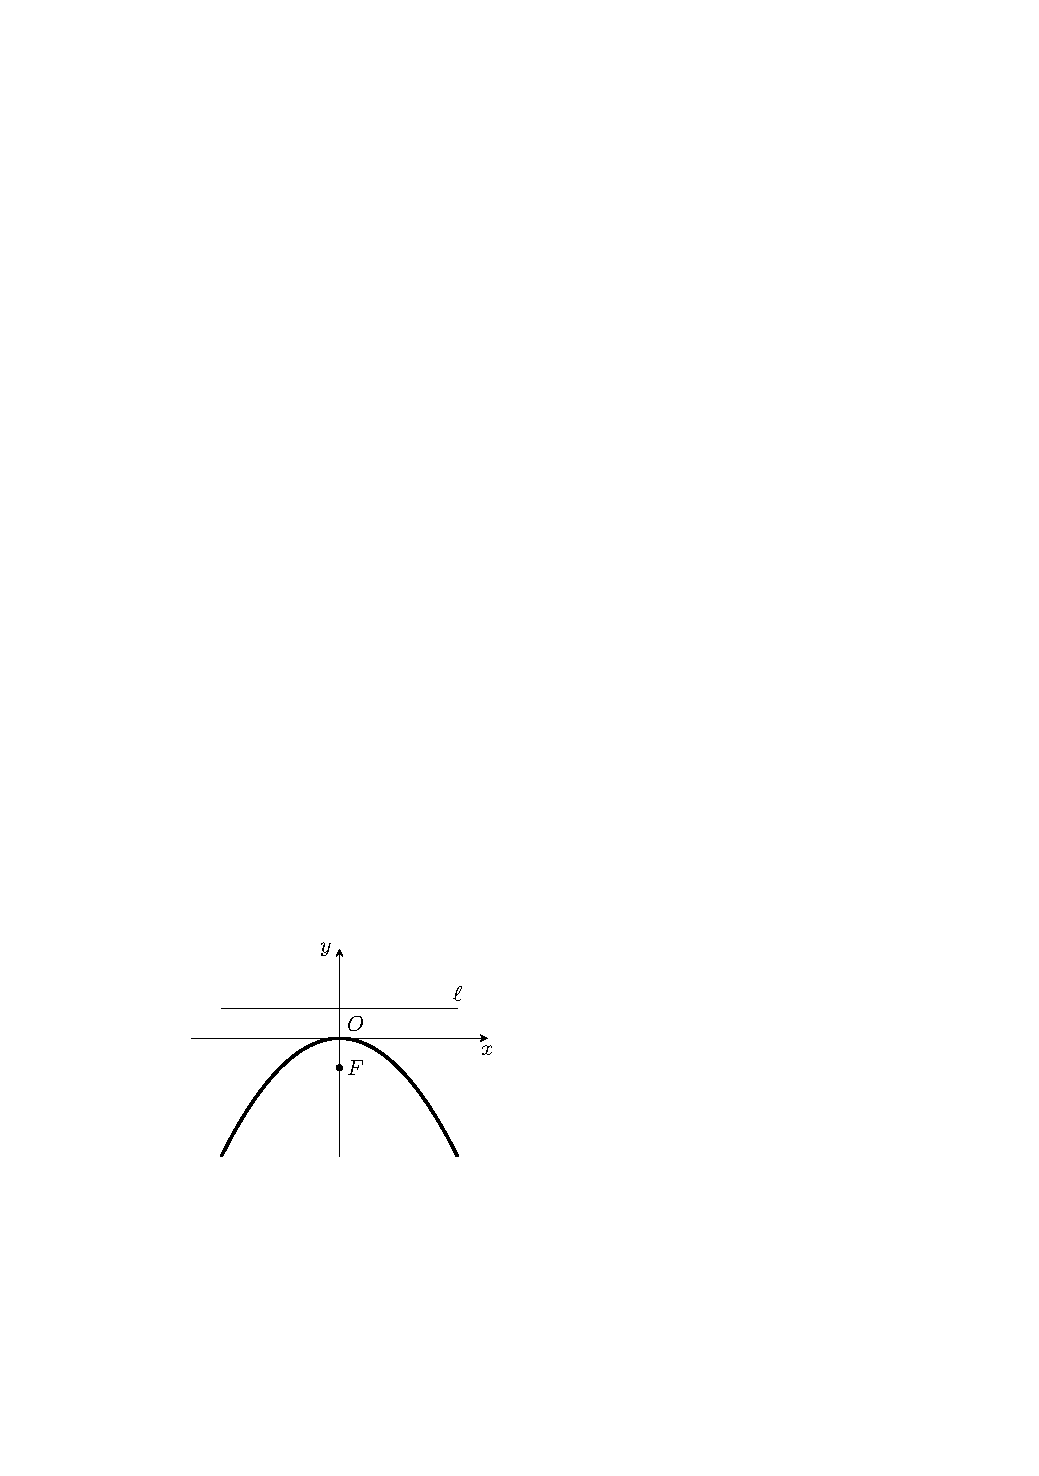
\includegraphics[scale=.7]{fig/para4.pdf} \\
\hline
\end{tabular}
\end{center}

我们可用同样的方法证明上述结论.

\begin{example}
    求下列抛物线的焦点坐标和准线方程：
\begin{multicols}{2}
\begin{enumerate}[(1)]
 \item $y^2=6x$;
\item $9x^2+2y=0$. 
\end{enumerate}
\end{multicols}
\end{example}

\begin{solution}
\begin{enumerate}[(1)]
\item 由标准方程可得$p=3$，开口向右，

$\therefore\quad $焦点坐标是$\left(\frac{3}{2},\; 0\right)$，准线方程是$x=-\frac{3}{2}$.
\item 由方程得标准方程$x^2=-\frac{2}{9}p$, $p=\frac{1}{9}$，开口向下，

$\therefore\quad $焦点坐标是$\left(0,\;-\frac{1}{18}\right)$，准线方程是$y=\frac{1}{18}$.
\end{enumerate}

\end{solution}

\begin{remark}
    在解决关于抛物线的问题时，抛物线的焦点与准线的距离$p\; (p>0)$，起着十分重要的作用. 在解题时，联想它的图形，有利于我们准确、迅速地得到正确的答案.
\end{remark}


\begin{example}
    根据下列条件，求出抛物线的标准方程：
\begin{multicols}{2}
\begin{enumerate}[(1)]
 \item 焦点是$F(-2,0)$；   \item 过点$A(4,-2)$
\end{enumerate}
\end{multicols}
\end{example}

\begin{analyze}
    由于抛物线的标准方程有四种，所以首先要确定是哪一种标准方程，然后再确定$p$值.
\end{analyze}

\begin{solution}
\begin{enumerate}[(1)]
    \item 因为焦点在$x$轴的负半轴上，并且$\frac{p}{2}=2$, $p=4$，所以它的标准方程是\[y^2=-8x\]

\noindent
\begin{minipage}{.47\textwidth}
    \item 因为点$A$在第四象限、满足条件的抛物线有两种（图3.41），所以设它的标准方程为
    $$y^2=2px\quad \text{和}\quad  x^2=-2py\; (p>0)$$

$\because\quad$    抛物线过点$A(4,-2)$,

$\therefore\quad $当$4=8p$时，得$p=\frac{1}{2}$；

当$16=4p$时，$p=4$.

$\therefore\quad$抛物线的标准方程是$y^2=x$和$x^2=-8y$.
\end{minipage}
\hfill
\begin{minipage}{.5\textwidth}
\centering
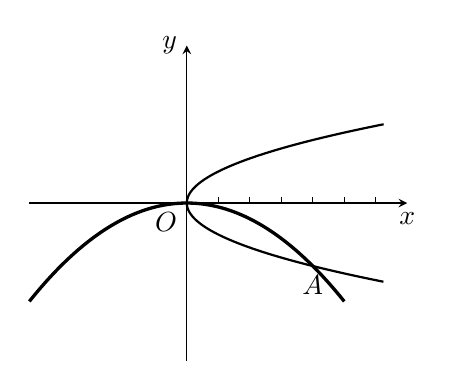
\begin{tikzpicture}[>=stealth, scale=.4]
\draw[->](-5,0)--(7,0)node[below]{$x$};
\draw[->](0,-5)--(0,5)node[left]{$y$};
\node[below left]{$O$};

\draw[domain=2.5:-2.5, thick, smooth, samples=100]plot({\x*\x} , \x);
\draw[domain=5:-5, very thick, smooth, samples=100]plot(\x, -.125*\x*\x);
\foreach \x in {1,2,...,6}
{
    \draw(\x,0)--(\x,.2);
}
\node at (4,-2)[below]{$A$};
\end{tikzpicture}
\captionof{figure}{}
\end{minipage}
\end{enumerate}
\end{solution}


\begin{example}
    已知抛物线的准线是直线$\ell:\; x+y+3=0$，焦点是点$F(1,4)$，求抛物线的方程．
\end{example}

\begin{analyze}
    很明显，抛物线的方程不是标准方程，不能用待定系数法. 这时应依据抛物线的定义求轨迹方程.
\end{analyze}



\begin{solution}
设抛物线上的动点为$P(x,y)$，由抛物线的定义可知，抛物线就是点集
\[M\left\{\text{点}P\Big| |PF|=d_{F-\ell}\right\}\]

$\therefore\quad \sqrt{(x-1)^2+(y-4)^2}=\frac{|x+y+3|}{\sqrt{2}}$

方程两边平方，并化简得
\[x^2-2xy+y^2-10x-22y+25=0\]
由于方程变形是同解变形，所以这就是所求的抛物线方程.
\end{solution}

\subsection*{3.15 练习}
\begin{enumerate}
\item 根据下列条件，写出抛物线的标准方程：
\begin{multicols}{2}
\begin{enumerate}[(1)]
    \item 焦点是$F(3,0)$;
    \item 准线方程是$y=-\frac{1}{4}$;
    \item 焦点到准线的距离是2．
\end{enumerate}
\end{multicols}

\item 求下列抛物线的焦点坐标和准线方程：
\begin{multicols}{2}
\begin{enumerate}[(1)]
    \item $y^2=20x$
    \item $y=2x^2$
    \item $2y^2-5x=0$
    \item $x^2+8y=0$
\end{enumerate}
\end{multicols}

\item 已知抛物线的焦点$F(1,1)$，准线方程$x+y+1=0$，求抛物线的方程.
\end{enumerate}

\section{抛物线的几何性质}
读者可根据抛物线的标准方程
\begin{equation}
    y^2=2px\quad (p>0) \tag{1}
\end{equation}
研究它的几何性质. 结论如下：

\begin{enumerate}
    \item 几何特性：若点$P$在抛物线上，则$\frac{|PF|}{d_{P-\ell}}=1$（$F\left(\frac{p}{2},\; 0\right)$是抛物线焦点）.
    \item 范围：
    抛物线在$y$轴的右侧，而且抛物线向右上方和右下方无限延伸.
    \item 对称性：
    抛物线关于$x$轴对称. 我们把抛物线的对称轴叫做抛物线的轴.
    \item 截距：
    抛物线的横、纵截距都为零，即抛物线过原点. 抛物线和它的轴的交点叫做抛物线的\textbf{顶点}. 抛物线$y^2=2px\; (p>0)$的顶点就是坐标原点.
    \item 离心率：
    抛物线上点$M$与焦点和准线的距离比，叫做抛物线的\textbf{离心率}，用$e$表示. 根据抛物线的定义，$e=1$
\end{enumerate}

    综上所述，方程$y^2=2px\; (p>0)$的曲线是：顶点在原点，开口向右，焦点为$F\left(\frac{p}{2},0\right)$，准线为直线$x=-\frac{p}{2}$的抛物线.

    对于抛物线的其他三种标准方程，用同样的方法可得到对应的几何性质.

\begin{example}
    已知抛物线的轴是$y$轴，它的顶点是坐标原点，并且经过点$M(2\sqrt{2},-2)$. 求它的标准方法，并用描点法画出图形.
\end{example}

\begin{solution}
    因为抛物线的轴为$y$轴，它的顶点是坐标原点，并且经过点$M(2\sqrt{2}-2)$，所以设它的标准方程为  
\[x^2=-2py\quad (p>0)\]
因为点$M$在抛物线上，所以
\[\left(2\sqrt{2}\right)^2=-2p\cdot (-2)\]
即：$p=2$，因此所求方程是$x^2=-4y$.

根据抛物线$x^2=-4y$的几何性质，利用$y=-\frac{x^2}{4}\; (x\ge 0)$计算抛物线在第四象限内的几个点的坐标，得
\begin{center}
    \begin{tabular}{c|cccccc}
\hline
$x$ &0&1&2&3&4&$\cdots$\\
\hline
$y$&0&$-0.25$&$-1$&$-2.25$&$-4$&$\cdots$\\
\hline
    \end{tabular}
\end{center}

描点画出抛物线在第四象限的一部分，再利用对称性，就可画出抛物线的另一部分（图3.42）．
\end{solution}


\noindent
\begin{minipage}{.5\textwidth}
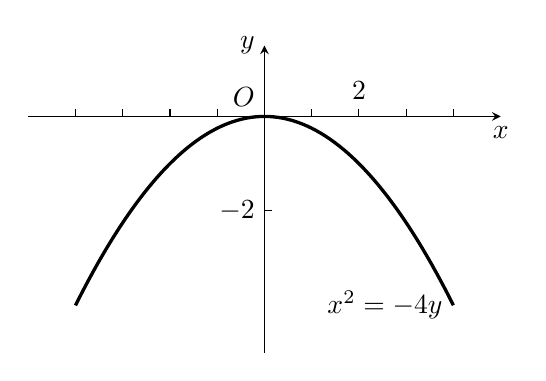
\begin{tikzpicture}[>=stealth, scale=.6]
\draw[->](-5,0)--(5,0)node[below]{$x$};
\draw[->](0,-5)--(0,1.5)node[left]{$y$};
\node[above left]{$O$};
\draw[domain=-4:4, smooth, samples=100, very thick]plot(\x, -0.25*\x*\x)node[left]{$x^2=-4y$};
\tkzDefPoints{0/0/A, 1/-.25/B, 2/-1/C, 3/-2.25/D, 4/-4/E}
\tkzDrawPoints(A,B,C,D,E)
\foreach \x in {1,2,...,4}
{
    \draw(\x,0)--(\x,.15);
    \draw(-\x,0)--(-\x,.15);
}
\node at (2,.15)[above]{2};
\draw(0,-2)node[left]{$-2$}--(.15,-2);


\end{tikzpicture}
\captionof{figure}{}
\end{minipage}
\hfill
\begin{minipage}{.45\textwidth}
\centering
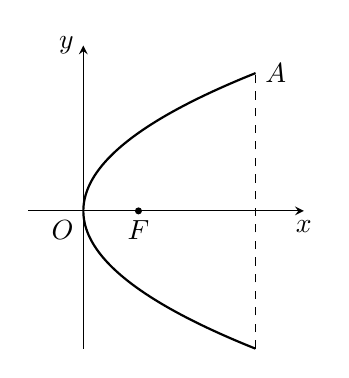
\begin{tikzpicture}[>=stealth, scale=.7]
\draw[->](-1,0)--(4,0)node[below]{$x$};
\draw[->](0,-2.5)--(0,3)node[left]{$y$};
\node[below left]{$O$};
\draw[domain=2.5:-2.5, thick, smooth, samples=100]plot({.5*\x*\x} , \x);
\draw[dashed](3.125,-2.5)--(3.125,2.5)node[right]{$A$};
\draw[fill](1,0)node[below]{$F$} circle(1.5pt);
\end{tikzpicture}
\captionof{figure}{}
\end{minipage}

\begin{example}
    探照灯反射镜的纵断面是抛物线的一部分．灯口直径是60cm，灯深40cm．求抛物线的标准方程和焦点的位置．
\end{example}

\begin{solution}
 在纵断面内，以反射镜的顶点（即抛物线的顶点）为
坐标原点，过顶点垂直于灯口直径的直线为$x$轴，建立直角坐标系（图3.43）．

设抛物线的标准方程是$y^2=2px$. 因为点$A$的坐标是$(40,30)$，代入方程，得
\[30^2=2p\cdot 40\]
即$p=\frac{45}{4}$，
所以抛物线的方程是$y^2=\frac{45}{2}x$，焦点坐标是$\left(\frac{45}{8},\; 0\right)$.
\end{solution}

\subsection*{3.16 练习}
\begin{enumerate}
\item 求适合下列条件的抛物线方程：
\begin{enumerate}[(1)]
\item 顶点在原点，关于$x$轴对称，并且经过点$M(5,-4)$;
\item 焦点是$F(0,-8)$，准线是$y=8$;
\item 顶点在原点，$y$轴是对称轴，且焦点到准线的距离为4；
\item 顶点在原点，坐标轴是对称轴，过点$(-1,2)$．
\end{enumerate}

\item 一条隧道的顶部是抛物拱形，拱高是1.1米，跨度是2.2米．求拱形的抛物线方程.
\item 根据抛物线的定义证明：函数$y=ax^2\; (a\ne 0)$的图象是抛物线.
\end{enumerate}

\section{抛物线的参数方程}
根据抛物线$y^2=2px\; (p>0)$的方程的特点：$x$是一次的、$y$是二次的，可设$x=2pt^2\; (t\in\R)$，由此得到
\[\begin{cases}
    x=2pt^2 \\
    y=2pt 
\end{cases}(t\in\R)\]
可以证明，它是抛物线$y^2=2px\; (p>0)$的一种参数方程，参数为$t$.

参数$t$的几何意义是，设抛物线上一点$P$，$OP$的斜率为$k_{OP}$，那么$t=\frac{1}{k_{OP}}$.

抛物线的参数方程的引入，也是为了给出抛物线上任一点的坐标，即抛物线$y^2=2px\; (p>0)$上的任意一点的坐标是$(2pt^2,2pt)$.

\begin{example}
    已知抛物线$y^2=2px\; (p>0)$, $p$为抛物线上的动点，定点$M(-1,0)$, $Q$点为有向线段$MP$上的定比分点，定比$\lambda=2$. 求动点$Q$的轨迹方程.
\end{example}

\begin{analyze}
    根据题目条件，解决问题的关键是如何确定$P$点的坐标. 此时，利用抛物线参数方程，是比较简便的方法.
\end{analyze}

\begin{solution}
由抛物线$y^2=2px\; (p>0)$可得其参数方程
\[\begin{cases}
    x=2pt^2\\ y=2pt
\end{cases}\]
则抛物线上的动点$P$的坐标为$(2pt^2,2pt)\; (t\in\R)$

设点$Q$的坐标为$(x,y)$,

$\because\quad \frac{MQ}{QP}=\lambda=2$

$\therefore\quad \begin{cases}
    x=\frac{-1+4pt^2}{3}\\[1.5ex]
    y=\frac{4pt}{3} 
\end{cases}(t\in\R)$

这就是点$Q$的轨迹的参数方程. 消去参数$t$就得到点$Q$的轨迹的普通方程
\[y^2=\frac{4p}{9}(3x+1)\]
\end{solution}

\begin{example}
 已知抛物线$y^2=2px\; (p>0)$与垂直于$x$轴的直线$\ell$交于$A$、$B$两点，$P$为抛物线上任一点，直线$AP$、$BP$分别交$x$轴于$M$、$N$两点（图3.44).

求证：$MN$的中点为定点.
\end{example}

\begin{proof}
$\because\quad A$、$B$、$P$在抛物线上，且$A$、$B$对称于$x$轴，


\noindent
\begin{minipage}{.52\textwidth}\CTEXindent
$\therefore\quad $设$A(2pt^2,2pt)$, $B(2pt^2,-2pt)$, $C(2pt_1^2,2pt_1)$，
则直线$AP$的方程是
\[y-2pt_1=\frac{2pt-2pt_1}{2pt^2-2pt^2_1}(x-2pt^2_1)\]
即
\[y-2pt_1=\frac{1}{t+t_1}(x-2pt^2_1)\]

令$y=0$，得$x=-2ptt_1$, 
\end{minipage}
\hfill
\begin{minipage}{.45\textwidth}
\centering
\begin{tikzpicture}[>=stealth, scale=.7]
\draw[->](-2,0)--(4,0)node[below]{$x$};
\draw[->](0,-2.5)--(0,3.5)node[left]{$y$};
\node[above left]{$O$};
\draw[domain=-2.5:2.5, thick, smooth, samples=100]plot({.5*\x*\x} , \x)node[right]{$y^2=2px$};
\tkzDefPoints{2/2/A, 2/-2/B, .5/-1/P}
\tkzDrawLines[add=.3 and .15](A,B)
\tkzDrawLines[add=1.3 and .5](P,B)
\tkzDrawLines[add=0 and 0](A,P)
\tkzLabelPoints[below right](A)
\tkzLabelPoints[above right](B)

\tkzDefPoints{-2/0/E, 2/0/F}
\tkzInterLL(B,P)(E,F) \tkzGetPoint{N}
\tkzInterLL(A,P)(E,F) \tkzGetPoint{M}
\tkzLabelPoints[below](P,M,N)
\tkzDrawPoints(N,O,M)
\node at (2,3.2)[right]{$\ell$};
\end{tikzpicture}
\captionof{figure}{}
\end{minipage}

$\therefore\quad $点$M$的坐标为$(-2ptt_1,0)$. 同理可得，点$N$的坐标为$(2ptt_1,0)$

$\therefore\quad MN$的中点坐标为$(0,0)$，
即：$MN$的中点为定点，即坐标原点.
\end{proof}

\subsection*{3.17 练习}
\begin{enumerate}
\item 连结原点$O$与抛物线$y=\frac{1}{2}x^2$上的动点$M$，延长$OM$至$P$，使$|OM|= |MP|$，求$P$点的轨迹的普通方程.
\item \begin{enumerate}[(1)]
    \item 从抛物线$y^2=2px$上各点，作$x$轴的垂线段，求线段
    中点的轨迹；
    \item 求抛物线$y^2=2px$上各点与焦点连线中点的轨迹方程.
\end{enumerate}
\end{enumerate}


\section{抛物线与直线}
抛物线与直线的位置关系，按公共点的个数分类，有三种：无公共点（相离）、一个公共点、两个公共点（相交）. 当有一个公共点时，又有两种情况：抛物线在直线$\ell$的一侧、抛物线在直线$\ell$的两侧（图3.45）．

\begin{figure}[htp]
    \centering
\begin{tikzpicture}[scale=.8]
\begin{scope}
    \draw[domain=-1.5:1.5, smooth, samples=100]plot({\x*\x} , \x);
    \draw[domain=2.5:-1.5, thick, smooth]plot(\x, {0.5*(\x+1)})node[below]{$\ell$};
\end{scope}
\begin{scope}[xshift=6cm]
    \draw[domain=-1.5:1.5, smooth]plot({\x*\x} , \x);
    \draw[thick](-1,0)--(3,0)node[below]{$\ell$};
\end{scope}    
\end{tikzpicture}
    \caption{}
\end{figure}

在建立适当坐标系后，设抛物线的方程为$y^2=2px\; (p>0)$，直线方程为$Ax+By+C=0\; (A^2+B^2\ne 0)$，这时，抛物线与直线的位置关系可通过方程组
$\begin{cases}
    y^2=2px\\
    Ax+By+C=0
\end{cases}$
的解的个数进行讨论.

\begin{enumerate}[(1)]
\item 方程组无实数解$\Longleftrightarrow$抛物线与直线相离．
\item 方程组有两个相同的实数解$\Longleftrightarrow$抛物线与直线有一个公共点（或者说，两个交点相重合，简称二重点）.

此时，我们把抛物线与直线的位置关系叫\textbf{相切}. 直线叫抛物线的\textbf{切线}，公共点叫\textbf{切点}.
\item 方程组有一个实数解$\Longleftrightarrow$抛物线与直线有一个公共点. 为区别于相切的位置关系，此时我们称抛物线与直线相交于一点.
\item 方程组有两个不相同的实数解$\Longleftrightarrow$抛物线与直线相交于两点.
\end{enumerate}

两个端点都在抛物线上的线段叫做抛物线的\textbf{弦}. 通过抛物线焦点的弦，叫做\textbf{过焦点的弦}. 垂直于抛物线的轴且过焦点的弦，叫做抛物线的\textbf{通径}.

\begin{example}
    已知抛物线$C:\; y^2=2px\; (p>0)$，直线$\ell:\; y=kx+b$，求抛物线$C$与直线$\ell$相切于一点和相交于一点的条件.
\end{example}

\begin{solution}
\[\begin{cases}
    y^2=2px\\ y=kx+b
\end{cases}\]
代入消元得
\[(kx+b)^2=2px \quad \Rightarrow\quad k^2x^2+2(kb-p)x+b^2=0\]
\[\begin{split}
\text{抛物线与直线相切于一点} &\Longleftrightarrow \text{方程组有两个相同的实数解}\\
&\Longleftrightarrow k\ne 0\; \text{且}\; \Delta=4(kb-p)^2-4k^2b^2=0\\
&\Longleftrightarrow k\ne 0\; \text{且}\; p(p-2kb)=0
\end{split}\]

$\because\quad p>0$,

$\therefore\quad $抛物线$C$与直线$\ell$相切于一点的充要条件是$k\ne 0$且$p-2kb=0$.

\[\begin{split}
    \text{抛物线与直线相交于一点}&\Longleftrightarrow \text{方程组有一个实数解}\\
    &\Longleftrightarrow k= 0\; \text{且}\; kb-p\ne 0
\end{split}\]

$\because\quad $当$k=0$时，$kb-p=-p\ne 0$

$\therefore\quad$抛物线$C$与直线$\ell$相交于一点的充要条件是$k=0$. 此时，直线$\ell$平行于抛物线$C$的轴（$x$轴）.
\end{solution}

\begin{example}
    设$AB$是抛物线$C:\; y^2=2px\; (p>0)$的过焦点的弦，$A$、$B$两点的坐标为$(x_1,y_1)$, $(x_2,y_2)$（图3.46），
求证：
\begin{multicols}{2}
    \begin{enumerate}[(1)]
        \item $y_1y_2=-p^2$
        \item $x_1x_2=\frac{1}{4}p^2$
    \end{enumerate}
\end{multicols}
\end{example}

\begin{proof}
\begin{enumerate}[(1)]
    \item 当$AB$不垂直于$x$轴时，设$AB$的斜率为$k$且$k\ne 0$, 则    
\[AB:\quad y=k\left(x-\frac{p}{2}\right)\]

交点$A,B$的坐标满足方程组
\[\begin{cases}
    y^2=2px\\ y=k\left(x-\frac{p}{2}\right)
\end{cases}\]

$\because\quad p\ne 0$

$\therefore\quad x=\frac{y^2}{2p}$，代入消$x$得


\noindent
\begin{minipage}{.45\textwidth}
\[y=k\left(\frac{y^2}{2p}-\frac{p}{2}\right)\]
整理得
\[\frac{k}{2p}y^2-y-\frac{kp}{2}=0\]
由条件可知，$y_1$、$y_2$为方程的两根，

$\therefore\quad y_1y_2=-\frac{kp}{2}\cdot \frac{2p}{k}=-p^2$.

当$AB\bot x$轴时，$x_1=x_2=\frac{p}{2}$,

$\therefore\quad y^2=2p\cdot \frac{p}{2}$，即$y^2-p^2=0$

$\therefore\quad y_1y_2=-p^2$
\end{minipage}
\hfill
\begin{minipage}{.52\textwidth}
\centering
\begin{tikzpicture}[>=stealth, scale=.55]
\draw[->](-2,0)--(8,0)node[below]{$x$};
\draw[->](0,-4.75)--(0,4.75)node[left]{$y$};
\node[below left]{$O$};
\draw[domain=4.5:-4.5, smooth, thick, samples=100]plot({.25*\x*\x} , \x)node[right]{$y^2=2px$};
\tkzDrawPoint(1,0)
\draw[domain=-1:3.5, smooth, thick]plot(\x, 2*\x-2);
\node at (1,0)[above right=.2]{$F\left(\frac{p}{2},\; 0\right)$};
\tkzDefPoints{2.62/3.236/A, .38/-1.236/B}
\tkzDrawPoints(A,B)
\node at (A)[right]{$A(x_1,y_1)$};
\node at (B)[right]{$B(x_2,y_2)$};


\end{tikzpicture}
\captionof{figure}{}
\end{minipage}

综上所述，过焦点的弦$AB$有$y_1y_2=-p^2$.

\item $\because\quad A$、$B$为抛物线上的点，

$\therefore\quad y^2_1=2px_1,\quad y^2_2=2px_2$

$\therefore\quad x_1x_2=\frac{y^2_1y^2_2}{4p^2}=\frac{p^4}{4p^2}=\frac{p^2}{4}$
\end{enumerate}
\end{proof}

\begin{example}
    求证：以过抛物线焦点的弦$AB$为直径的圆，必与其准线相切.
\end{example}

\begin{analyze}
    证明直线与圆相切，方法较多.例如求出直线方程和圆的方程，证明由它们组成的方程组有两个相等的实数解；再如，求出弦的中点，证明它到准线距离等于弦长的一半，在解析几何中，我们往往想到用代数方法求弦长、求中点到准线的距离. 下面介绍利用抛物线的几何特征证明此题的方法.
\end{analyze}

\begin{proof}
设弦$AB$的中点为$C$，抛物线的焦点为$F$.

欲证以$AB$为直径的圆与准线相切，只要证明点$C$到准线的距离等于$\frac{1}{2}|AB|$. 分别过$A$、$B$、$C$作准线的垂线$AA'$、$BB'$、$CC'$，垂足分别为$A'$、$B'$、$C'$，得到直角梯形$AA'B'B$（图3.47）．由抛物线的定义可知：

\noindent
\begin{minipage}{.53\textwidth}

\[|AB|=|AF|+|BF|=|AA'|+|BB'|\]
所以，只要证
\[|CC'|=\frac{1}{2}(|AA'|+|BB'|)\]
由梯形性质可知
\[|CC'|=\frac{1}{2}(|AA'|+|BB'|)\]

$\therefore\quad$以过抛物线焦点的弦$AB$为直径的圆，必与其准线相切.
\end{minipage}
\hfill
\begin{minipage}{.45\textwidth}
\centering
\begin{tikzpicture}[>=stealth, scale=.8]
    \draw[->](-2,0)--(4,0)node[below]{$x$};
    \draw[->](0,-3)--(0,4)node[left]{$y$};
    \node[below left]{$O$};
    \draw[domain=3:-2.75, smooth, thick, samples=100]plot({.25*\x*\x} , \x);
\draw(-1,3.5)node[above]{$\ell$}--(-1,-3);
\draw[domain=.61:1.64, smooth, thick]plot(\x, 4*\x-4);
\tkzDefPoints{1.64/2.56/A, 0.61/-1.56/B, -1/4/M}
\tkzDefPoints{-1/2.56/A', -1/-1.56/B'}
\tkzDefMidPoint(A,B) \tkzGetPoint{C}
\tkzDefMidPoint(A',B') \tkzGetPoint{C'}
\tkzDrawPolygon(A,A',B',B)
\tkzDrawSegments(C,C')
\tkzLabelPoints[left](A',B',C')
\tkzLabelPoints[right](A,B,C)
\node at (1,0)[below right]{$F$};
\tkzMarkRightAngles[size=.2](M,A',A M,B',B M,C',C)
\tkzDrawPoint(1,0)
\end{tikzpicture}
\captionof{figure}{}
\end{minipage}
\end{proof}

\begin{example}
已知直线$\ell:\; y=mx+m$ ($|m|<1$且$m\ne 0$) 和抛物线$C:\; y^2=4x$.
\begin{enumerate}[(1)]
\item 求证：$\ell$与$C$必相交于两点；
\item 求截得的弦长；
\item 当$m$为何值时，弦的中点在直线$x-y-3=0$上．
\end{enumerate}
\end{example}

\begin{solution}
\begin{enumerate}[(1)]
    \item 解方程组$\begin{cases}
        y=mx+m\\ y^2=4x
    \end{cases}$代入消$y$整理得
\begin{equation}
    m^2x^2+2(m^2-2)x+m^2=0 \tag{1}
\end{equation}

$\because\quad m\ne 0$

$\therefore\quad \Delta =4(m^2-2)^2-4m^2\cdot m^2=16(1-m^2)$    

$\because\quad |m|<1,\quad 1-m^2>0$
    
$\therefore\quad \Delta >0$，$\ell$与$C$必相交于两个点.

\item 设交点为$A(x_1,y_1)$，$B(x_2,y_2)$.
\[|AB|=\sqrt{(x_1-x_2)^2+(y_1-y_2)^2}\]

$\because\quad y_1=mx_1+m,\quad y_2=mx_2+m$

\[\begin{split}
    \therefore\quad |AB|=\sqrt{1+m^2}\cdot |x_2-x_1|
&=\sqrt{1+m^2}\cdot \frac{\sqrt{\Delta }}{m^2}\\
&=\sqrt{1+m^2}\cdot \frac{\sqrt{16(1-m^2)}}{m^2}\\
&=\frac{4}{m^2}\sqrt{1-m^4}
\end{split}\]

\item 设$AB$的中点为$C(x_0,y_0)$，则
\[\begin{split}
  x_0&=\frac{x_1+x_2}{2}=\frac{2-m^2}{m^2}\\
y_0&=\frac{y_1+y_2}{2}=\frac{m(x_1+x_2)+2m}{2}=\frac{2}{m}  
\end{split}\]

要使点$C$在直线$x-y-3=0$上，只要
\[\frac{2-m^2}{m^2}-\frac{2}{m}-3=0\]
解得：$m=\frac{1}{2},\quad m=-1$（舍）.

$\therefore\quad $当$m=\frac{1}{2}$时，$AB$的中点在直线$x-y-3=0$上．
\end{enumerate}
\end{solution}

\begin{remark}
此题中，着重介绍了求圆锥曲线的弦长、弦的中点坐标的常用方法. 直线$y=kx+b$上两点$A(x_1,y_1)$，$B(x_2,y_2)$的距离公式
\[|AB|=\sqrt{1+k^2}\cdot |x_2-x_1|=\sqrt{1+k^2}\sqrt{(x_1+x_2)^2-4x_1x_2}\]
可作为公式使用.

另外，若$x_1,x_2$是方程$ax^2+bx+c=0$的两个根，则
\[|x_2-x_1|=\frac{\sqrt{b^2-4ac}}{|a|}\]
\end{remark}

\subsection*{3.18 练习}
\begin{enumerate}
\item $AB$是抛物线$y^2=2px\; (p>0)$的过焦点$F$的弦，$|FA|$、$|FB|$叫做抛物线的焦半径.
\begin{enumerate}[(1)]
\item 求焦半径$|FA|$;
\item 求弦长$|AB|$;
\item 证明：通径是最短的过焦点的弦．
\end{enumerate}    


\item 已知直线$\ell:\; y=2x+m$与抛物线$y=-\frac{1}{2}x^2+6$相交于$A$、$B$两点，

求$m$为何值时$|AB|=2\sqrt{5}$.
\item 已知抛物线$y^2=2x$，过定点$Q(2,1)$作直线$\ell$交抛物线于$A$、$B$两点，求弦$AB$中点$P$的轨迹方程.
\end{enumerate}

\section*{习题六}
\begin{center}
    \bfseries A
\end{center}

\begin{enumerate}
  \item 求下列抛物线的焦点坐标和准线方程：
\begin{multicols}{2}
\begin{enumerate}[(1)]
  \item $x^2=-\frac{1}{4}y$
\item $2x^2-3y=0$
\item $3x+2y^2=0$
\item $5y^2-4x=0$ 
\end{enumerate}
\end{multicols}

\item 求适合下列条件的抛物线的方程：
\begin{enumerate}[(1)]
\item 顶点在原点，焦点是$F(0,5)$;
\item 顶点在原点，准线是直线$y=4$;
\item 顶点在原点，对称轴是$x$轴，并且顶点与焦点的距离等于6；
\item 顶点在原点，对称轴是$y$轴，并且焦点到准线的距离等于4．
\end{enumerate}  

\item \begin{enumerate}[(1)]
    \item  抛物线$y^2=2px\; (p>0)$上点$M$到焦点$F$的距离为$a$，求点$M$的横坐标和$a$的取值范围.
    \item 求与$x$轴相切于原点，在抛物线$y=ax^2\; (a>0)$的内部，且面积最大的圆的方程.
\end{enumerate} 

\item 在抛物线$y^2=12x$上，求和焦点的距离等于9的点的坐标．
\end{enumerate}

\begin{center}
    \bfseries B
\end{center}

\begin{enumerate}\setcounter{enumi}{4}
    \item 有一正三角形的两个顶点在抛物线$y^2=2px$上，另一顶点在原点. 求这个三角形的边长.
    \item 图中是抛物线形拱桥，当水面在$\ell$时，拱顶离水面2米，水面宽4米。水下降1米后，水面宽多少？
\begin{figure}[htp]
    \centering
\begin{tikzpicture}[>=stealth]
\draw[domain=-1.2:1.2, smooth, thick, pattern=bricks]plot(\x, -\x*\x)--(2,-1.44)--(2,.5)--(-2,.5)--(-2,-1.44)--(-1.2,-1.44)--cycle;
\fill[cyan!20!white](-1.2,-1.44)--(-1,-1)node[above right=.1, black]{$\ell$}--(1,-1)--(1.2,-1.44)--cycle;
\draw(-1,-1)--(-1,-2);
\draw(1,-1)--(1,-2);
\draw[<->](1,-1.7)--node[fill=white]{4}(-1,-1.7);
\draw[|<->](0,-1)--node[fill=white]{2}(0,0);

\end{tikzpicture}
    \caption*{第6题}
\end{figure}
    \item 抛物线的顶点是双曲线$16x^2-9y^2=144$的中心，而焦点是双曲线的左顶点. 求抛物线的方程.
    \item 求过点$(0,2)$且被抛物线$y=\frac{1}{6}x^2+\frac{4}{3}$截得的弦长为$\frac{5\sqrt{5}}{2}$的直线.
    \item 已知直线$C_1:\; x=2$和圆$C_2:\; (x+4)^2+y^2=4$，设动圆与$C_1$相切、与$C_2$相外切，求动圆圆心$C$的轨迹．
    \item 抛物线$y^2=8x$的焦点为$F$，$A(4,-2)$为一定点在抛物线上找一点$M$，使$|MA|+|MF|$的值最小，求点$M$的坐标.
    \item 过抛物线焦点的一条直线与抛物线交于两点$P$、$Q$，通过点$P$和抛物线顶点的直线交准线于点$M$. 求证：直线$MQ$平行于抛物线的轴.
    \item 过抛物线$y^2=2px\; (p>0)$的顶点$O$任作互相垂直的两弦$OM$、$ON$，
    
    求证：$MN$交$x$轴于定点.
\end{enumerate}

\begin{center}
    \bfseries C
\end{center}
\begin{enumerate}\setcounter{enumi}{12}
\item $\triangle ABC$的三顶点都在以$x$轴为对称轴，原点为顶点的抛物线上，已知点$A(-2,4)$.
\begin{enumerate}[(1)]
\item 求抛物线的方程；
\item 若$\triangle ABC$的重心就是抛物线的焦点，求过$B$、$C$两点的直线方程.
\end{enumerate}

\item 过抛物线$y^2=2px$的顶点$O$任作互相垂直的两弦$OM$、$ON$，求$\triangle MON$面积的最小值和取最小值时$M$、$N$点的坐标.
\item 长为$\ell\; (\ell>1)$的线段$AB$的两个端点$A$、$B$在抛物线$y=x^2$上移动，求$AB$的中点$M$到$x$轴距离的最小值.
\end{enumerate}

\section{本章小结}
\subsection{本章主要内容}
\begin{enumerate}
\item 本章在第二章直线方程的基础上，研究了直角坐标系中曲线和方程之间的对应关系，然后根据所求曲线的定义，得出了几种圆锥曲线的方程，并通过方程讨论了圆、椭圆、双曲线和抛物线的性质及应用.
\item 根据圆的定义，求出了圆的标准方程，又由标准方程推出了圆的一般方程.圆的标准方程的优点，在于它明确地指出了圆心和半径，而圆的一般方程则突出了方程形式上的特点，它不含$xy$项，并且$x^2$、$y^2$项的系数相等.
\item 由椭圆、双曲线、抛物线的几何条件求其标准方程，并通过分析标准方程研究这三种曲线的几何性质. 三种曲线的标准方程（各取其中一种）和图形、性质如下表：
\end{enumerate}

\begin{center}
\begin{tabular}{cm{3cm}m{3cm}m{3cm}}
\hline
&椭圆&双曲线&抛物线\\ \hline
几何条件 & 与两个定点的距离和等于常数 &与两个定点的距离差的绝对值等于常数 &与一个定点和一条定直线的距离相等\\
\hline
标准方程& $\frac{x^2}{a^2}+\frac{y^2}{b^2}=1$& $\frac{x^2}{a^2}-\frac{y^2}{b^2}=1$& $y^2=2px$\\[1.5ex]
& $(a>b>0)$ & $(a>0,\; b>0)$ & $(p>0)$\\[1.5ex]
\hline
图形& 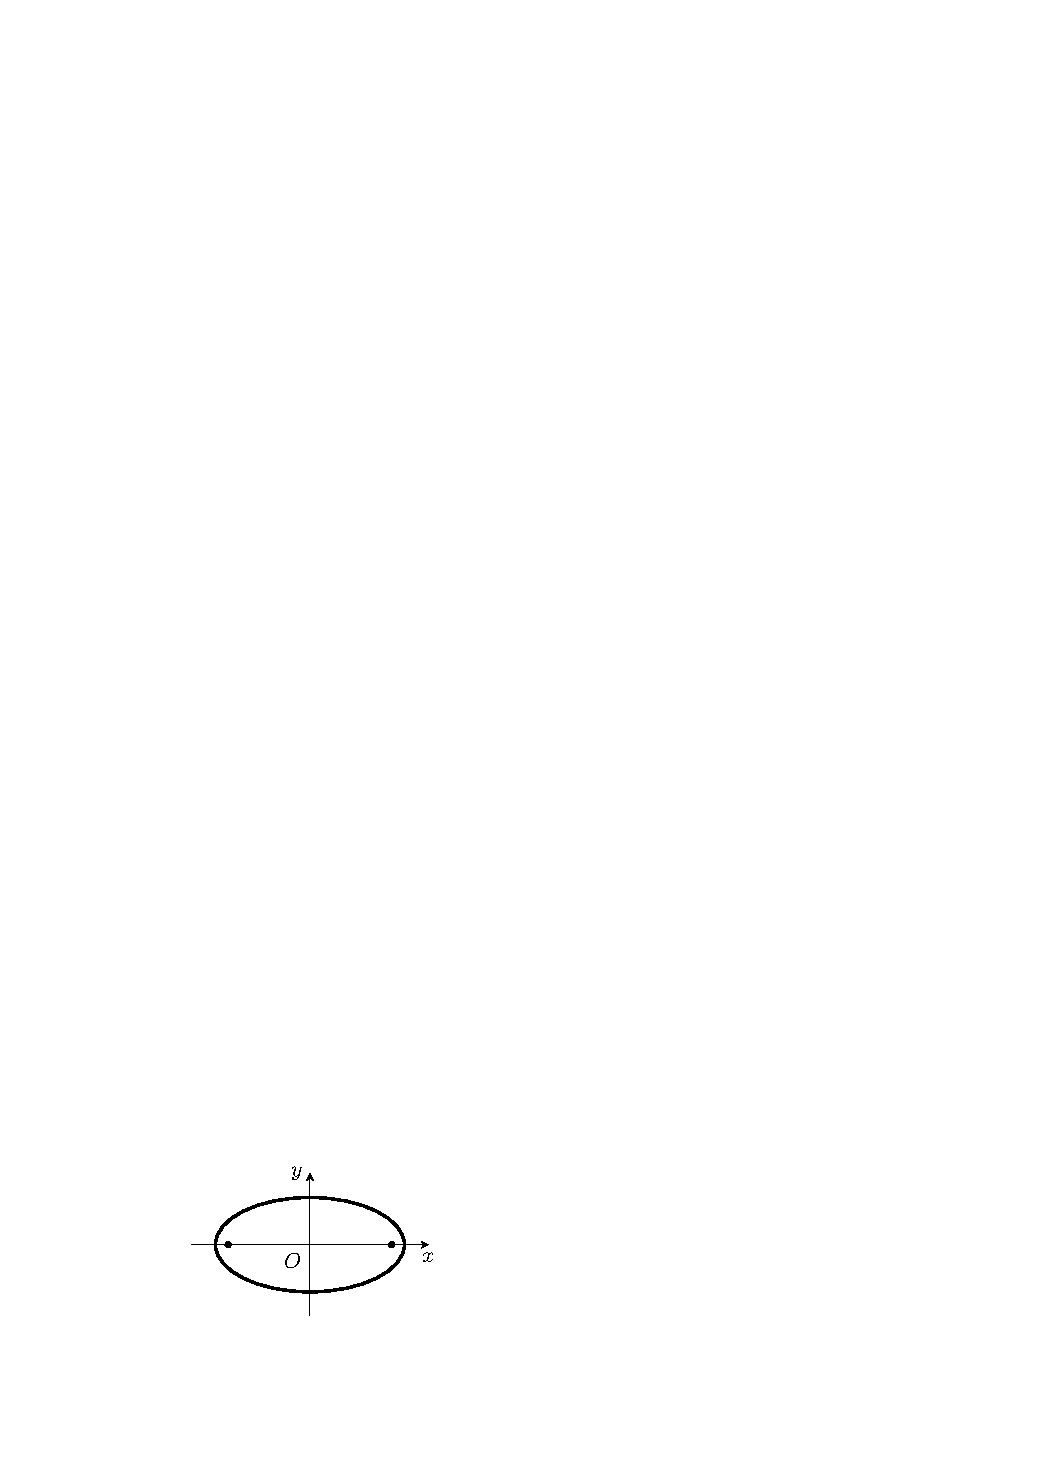
\includegraphics[scale=.6]{fig/ellip.pdf} &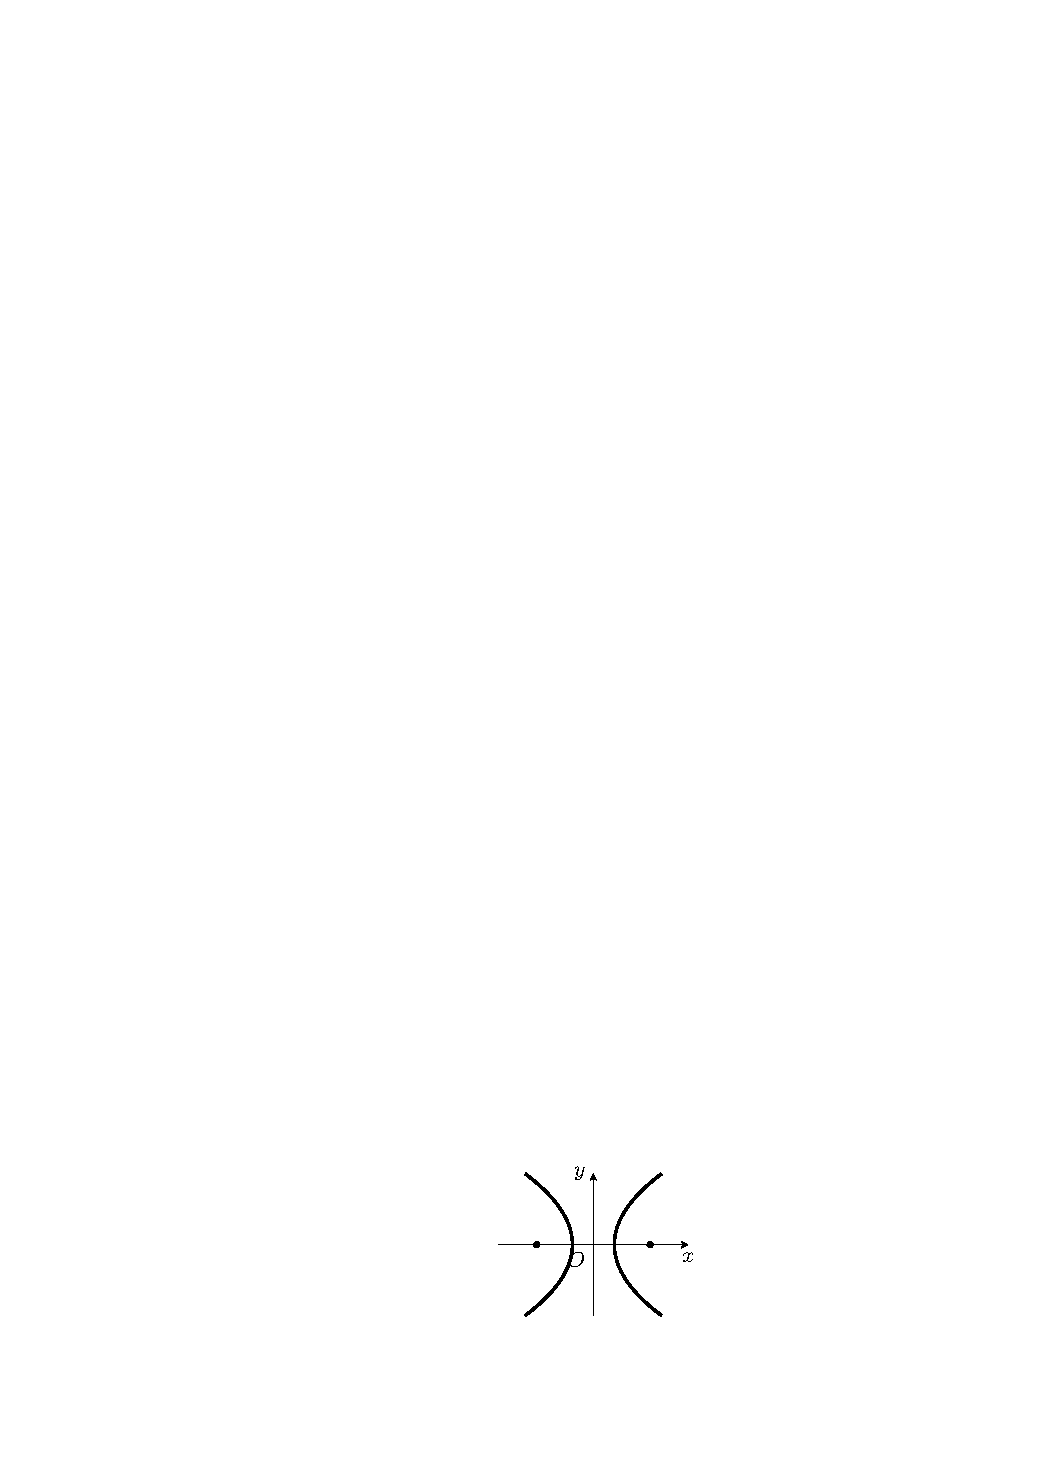
\includegraphics[scale=.6]{fig/hyper.pdf}&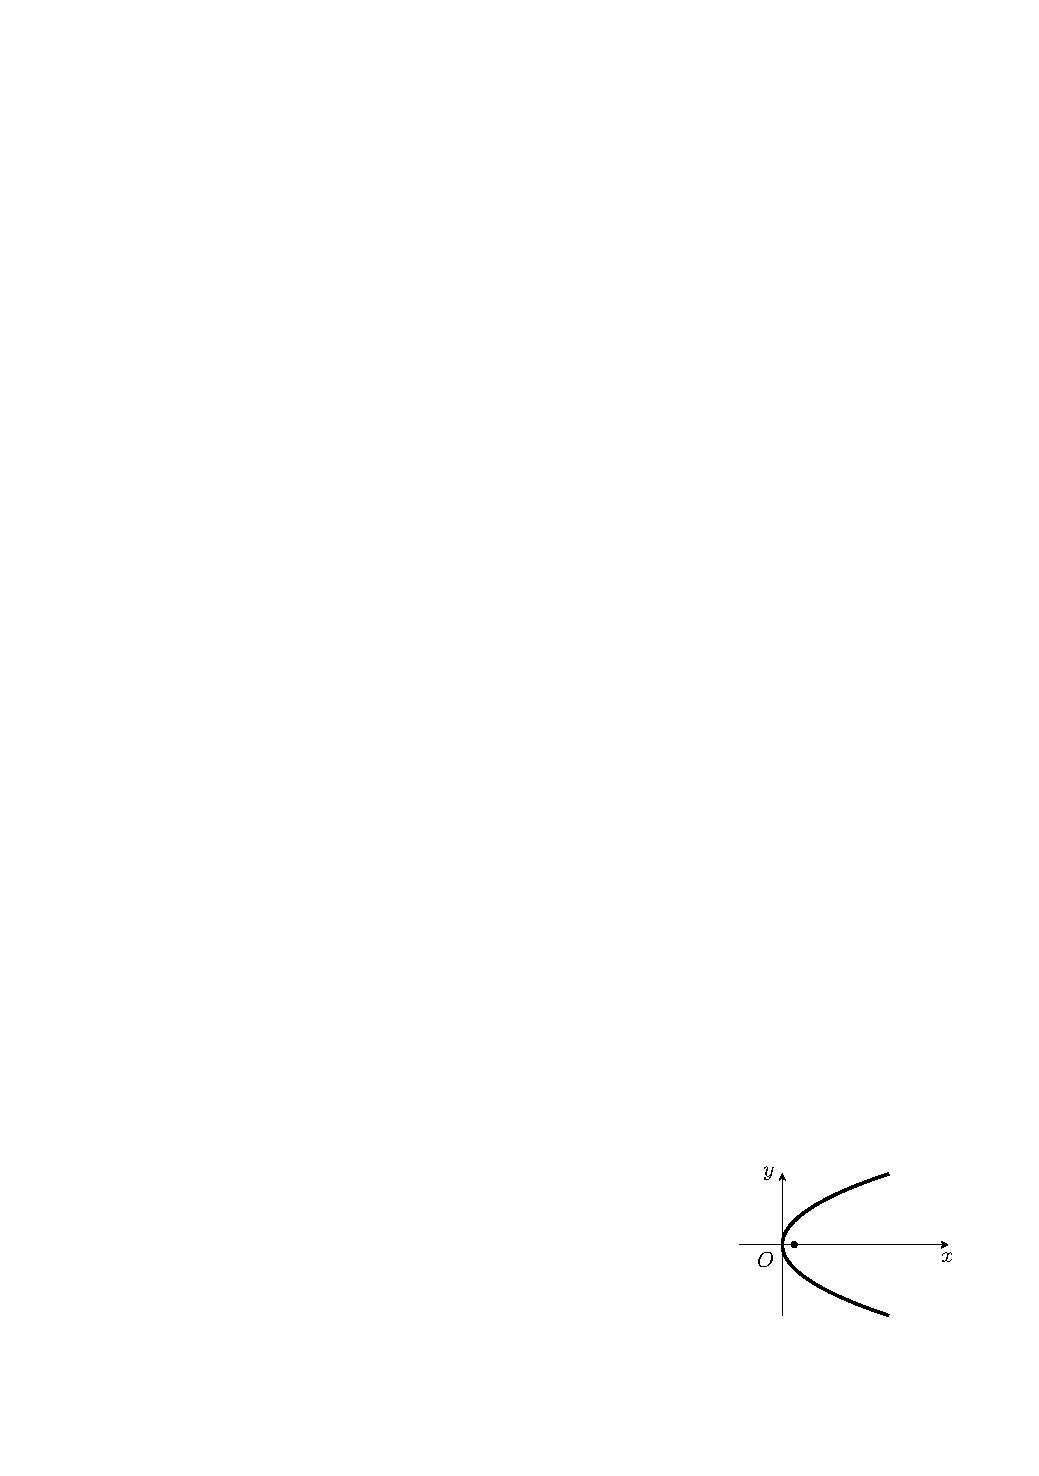
\includegraphics[scale=.6]{fig/para.pdf}\\  \hline
顶点坐标 & $(\pm a,0),\; (0,\pm b)$ &$(\pm a,0)$ & $(0,0)$\\
\hline
对称轴 & $x$轴．长轴长$2a$ &$x$轴．实轴长$2a$&$x$轴\\
&$y$轴．短轴长$2b$ &$y$轴．虚轴长$2b$&\\ \hline
焦点坐标 & $(\pm c,0)$& $(\pm c,0)$& $\left(\frac{p}{2},\; 0\right)$\\
& $c=\sqrt{a^2-b^2}$& $c=\sqrt{a^2+b^2}$\\[1.5ex] \hline
离心率 & $0<e<1$ & $e>1$ &$e=1$\\
\hline
准线& $x=\pm\frac{a^2}{c}$& $x=\pm\frac{a^2}{c}$& $x=-\frac{p}{2}$\\[1.5ex] \hline
渐近线&&$y=\pm\frac{b}{a}x$ & \\[1.5ex]
\hline
\end{tabular}
\end{center}

\subsection{圆、椭圆、双曲线、抛物线的统一性}
\begin{enumerate}
\item 从方程的形式看：在直角坐标系中，这几种曲线的
方程都是二元二次的，所以把它们称为二次曲线.
\item 除圆以外，从点的集合（或轨迹）的观点来看：它们都是与定点和定直线距离的比是常数$e$的点的集合（或轨迹），这个定点是它们的焦点，定直线是它们的准线. 只是由于离心率$e$的不同，而分为椭圆、双曲线和抛物线三种曲线.
\item 从天体运行的轨道看：天体运动的轨道是这四种曲线，例如，人造卫星、行星、彗星等由于运动的速度的不同，它们的轨道是圆、椭圆、抛物线或双曲线.
\item 四种曲线又可以看作不同的平面截圆锥面所得到的截线，因此，它们又统称圆锥曲线.
\end{enumerate}

\subsection{直线与圆锥曲线的位置关系}
\begin{enumerate}
  \item 直线与圆锥曲线的位置关系有三种，即相离、相切、相交.
\item 可以证明，过圆锥曲线上一点$P(x_0,y_0)$的切线方程如下表：
\end{enumerate}

\begin{center}
\begin{tabular}{cc}
   \hline
    圆锥曲线&  过曲线上一点$P(x_0,y_0)$的切线方程\\
    \hline
$x^2+y^2=r^2$  & $x_0y+y_0y=r^2$\\
$\frac{x^2}{a^2}+\frac{y^2}{b^2}=1$ & $\frac{x_0 x}{a^2}+\frac{y_0 y}{b^2}=1$\\[1.5ex]
$\frac{x^2}{a^2}-\frac{y^2}{b^2}=1$ & $\frac{x_0 x}{a^2}-\frac{y_0 y}{b^2}=1$\\[1.5ex]
$y^2=2px$ &$y_0 y=p(x+x_0)$\\
\hline
\end{tabular}
\end{center}

\subsection{直线和圆锥曲线的参数方程}
\begin{enumerate}
    \item 我们根据曲线的参数方程的概念，在建立直线及圆锥曲线的参数方程的过程中，都是根据所给曲线的性质，选择适当的变量作为参数，使得所选定的参数能刻划曲线上任
意一点$P$的位置，并且能比较容易建立这点的坐标$x$、$y$与参数之间的函数解析表达式.
\begin{enumerate}[(1)]
    \item 直线：经过点$P_0(x_0,y_0)$，倾斜角为$\alpha$的直线的参数方程是
\[\begin{cases}
    x=x_0+t\cos\alpha\\
    y=y_0+t\sin\alpha
\end{cases}\]
    其中$t$是参数，$t$表示直线上的定点$P_0(x_0,y_0)$到动点$P(x,y)$的有向线段$\overline{P_0P}$的数量. 一般规定，直线向上（或向右）的方向为有向直线的正方向.
    
    由于$\alpha$是直线的倾角，它的范围是$[0,\pi)$，故$\cos\alpha\in (-1,1]$, $\sin\alpha\in  [0,1]$.
\item 圆： 以$O(a,b)$为圆心，$r$为半径的圆的参数方程是
\[\begin{cases}
    x=a+r\cos\varphi\\
    y=b+r\sin\varphi
\end{cases}\]
    其中$\varphi$是参数，$\varphi$是以$x$轴正方向为始边，以从$O'(a,b)$出发过圆上动点$P(x,y)$的射线为终边所成的角，一般规定$\varphi \in[0,2\pi)$.
   \item 椭圆：中心在$O'(x_0,y_0)$，长半轴为$a$，短半轴为$b$，焦点在与$x$轴平行的直线上的椭圆参数方程为
\[\begin{cases}
    x=x_0+a\cos\varphi\\
    y=y_0+b\sin\varphi\\
\end{cases}\]
    其中$\varphi$是参数，它叫椭圆的离心率. $\varphi$的范围是$[0,2\pi)$.
 
    \item 双曲线：
    中心在$O'(x_0,y_0)$，实半轴为$a$，虚半轴为$b$，焦点在
与$x$轴平行的直线上的双曲线参数方程为
\[\begin{cases}
    x=x_0+a\sec\varphi\\
    y=y_0+b\tan\varphi\\
\end{cases}\]
其中$\varphi$为参数，它叫双曲线的离心角，$\varphi$的范围是
\[\left[0,\; \frac{\pi}{2}\right)\cup\left(\frac{\pi}{2},\; \frac{3\pi}{2}\right)\cup \left(\frac{3\pi}{2},\; 2\pi\right)\]
\item 抛物线：
顶点在$O(0,0)$，焦参数为$p$，开口方向向右的抛物线参数方程为
\[\begin{cases}
    x=2pt^2\\ y=2pt
\end{cases}\]
其中$t$是参数，$t$表示连结$O(0,0)$和抛物线上动点$P(x,y)$的直线斜率的倒数.
\end{enumerate}
\item 我们建立的直线和圆锥曲线的参数方程中，由于参数有比较明显的几何或物理意义，因此，利用它们解决一些解析几何问题时，有时要比用普通方程解决问题简便得多.
\end{enumerate}


\subsection{本章要注意运用和掌握的数学思想方法}
\begin{enumerate}
\item 数形结合思想；
\item 转化的思想；
\item 待定系数法、配方法、分析法等．
\end{enumerate}


\section*{复习题二}
\begin{center}
    \bfseries A
\end{center}

\begin{enumerate}
    \item 求和圆$x^2+y^2=25$外切于点$P(4,3)$，且半径是1的圆的方程.
    \item 求经过两圆$x^2+y^2=1$, $x^2+y^2-2x-2y+1=0$的交点的直线被圆$x^2+y^2=\frac{25}{4}$所截的弦长.
    \item 已知两条直线$\ell_1:\; 2x-3y+2=0$和$\ell_2:\; 3x-2y+3=0$，有一动圆$M$与$\ell_1$、$\ell_2$都相交，并且$\ell_2$被圆$M$所截的弦长分别是26、24，求圆心$M(x,y)$的轨迹方程.
    \item 已知椭圆$\frac{x^2}{a^2}+\frac{y^2}{b^2}=1\; (a>b>0)$，直线$\ell$过点$A(-a,0)$、$B(a,b)$，若直线$\ell$与椭圆还交于$C$点，求$|AC|:|BC|$.
    \item 过双曲线$x^2-y^2=8$的右焦点$F_2$有一条弦$PQ$，它的长为7，$F_1$是另一焦点，求$\triangle F_1PQ$的周长.
    \item 已知抛物线$y^2=2px$有一个内接直角三角形，直角顶点为坐标原点、一直角边所在直线方程为$y=2x$，斜边长为$5\sqrt{2}$，求这条抛物线的方程.
\end{enumerate}

\begin{center}
    \bfseries B
\end{center}

\begin{enumerate}\setcounter{enumi}{6}
    \item 过椭圆$\frac{x^2}{2}+y^2=1$的一个焦点$F$作直线$\ell$交椭圆于$A$、$B$，椭
    圆中心是原点$O$，当$\triangle AOB$面积最大时，求$\ell$的方程.
    \item 若正方形$ABCD$的一边$AB$在直线$x-2y+10=0$上，$C$、$D$点分别在椭圆$\frac{x^2}{16}+\frac{3y^2}{4}=1$上，求此正方形的边长.
    \item 已知双曲线$2x^2-y^2=2$，过点$A(\sqrt{3},0)$作直线$\ell$ 与此双曲线相交于$P$、$Q$两点，若$|PQ|$等于此双曲线实轴长的3倍，求$\ell$的倾斜角．
    \item 已知$\odot C$过定点$A(O,P)\; (P\in\R^+)$，圆心$C$在抛物线$x^2=2py$上运动，若$MN$为$\odot C$在$x$轴上截得的弦，设$|AM|=L_1$, $|AN|=L_2$, $\angle MAN=\theta$.
\begin{enumerate}[(1)]
 \item 当$C$点运动时，$|MN|$是否变化？写出并证明你的结论；
\item 求式子$\frac{L_2}{L_1}+\frac{L_1}{L_2}$的最大值，并求取得这个最大值时$\theta$的值和此时$\odot C$的方程.
\end{enumerate}

\item 如果抛物线$y^2=2px$和圆$(x-2)^2+y^2=3$相交，它们在$x$轴上方的交点为$A$、$B$，那么当$p$为何值时，线段$AB$的中点$M$在直线$y=x$上.
\item 从椭圆$\frac{x^2}{a^2}+\frac{y^2}{b^2}=1\; (a>b>0)$上一点$P$向$x$轴作垂线，垂足恰好是左焦点$F_1$，若点$A(a,0)$和点$B(0,b)$的连线$AB\parallel OP$，求此椭圆的离心率$e$.
\item 已知椭圆$x^2+\frac{y^2}{4}=1$及两点$P(-2,0)$、$Q(0,1)$，过点$P$作斜率为$k$的直线交椭圆于两点$A$、$B$，设线段$AB$的中点为$M$，连结$QM$.
\begin{enumerate}[(1)]
    \item $k$为何值时，直线$QM$与椭圆的准线平行；
    \item $k$为何值时，直线$QM$过椭圆的顶点．
\end{enumerate}
\end{enumerate}

\begin{center}
    \bfseries C
\end{center}

\begin{enumerate}\setcounter{enumi}{13}
    \item 已知双曲线$\frac{x^2}{a^2}-\frac{y^2}{b^2}=1\; (a>0,\; b>0)$左、右两个焦点分别为$F_1$、$F_2$，$P$是它左侧分支上一点，$P$到左准线的距离为$d$.
\begin{enumerate}[(1)]
 \item 若$y=\sqrt{3}x$是已知双曲线的一条渐近线，是否存在$P$点，使$d$、$|PF_1|$、$|PF_2|$成等比数列？若存在，写出$P$点坐标；若不存在，说明理由.
\item 在已知双曲线的左侧分支上，使$d$、$|PF_1|$、$|PF_2|$成
    等比数列的$P$点存在时，求离心率$e$的取值范围.  
\end{enumerate}

    \item 把椭圆$\frac{x^2}{a^2}+\frac{y^2}{b^2}=1$的长轴$n$等分，过每一个分点依次作长轴$A_1A_2$的垂线，分别交椭圆的上半部于$B_1,B_2,B_3,\ldots,B_{n-1}$. 若$F_1$是椭圆的左焦点，试求：
    \[|F_1A_1|+|F_1B_1|+|F_1B_2|+\cdots+|F_1B_{n-1}|+|F_1A_2|\]

\item 已知双曲线$x^2-y^2=a^2$，过点$B(0,-a)$双曲线右支的割线$BCD$、过焦点$F(c,0)$作平行于直线$BD$的直线交双曲线于$G$、$H$两点. 

求$\frac{|BC|\cdot |BD|}{|GF|\cdot |FH|}$的值.
\end{enumerate}